%%%COMPILED WITH XELATEX!%%%

%%%PREAMBLE%%%

%%%BASIC SETUP, COMPILED WITH XELATEX!%%%


\documentclass[10pt]{article}
\usepackage[margin=1.25in]{geometry}
\hyphenpenalty=5000
\usepackage{graphicx}
\usepackage{tabularx}
\usepackage[usenames,dvipsnames]{xcolor}
\usepackage{tikz}
\usepackage{longtable}
\usepackage{caption}
\usepackage{wrapfig}
\usepackage{booktabs, array}
\usepackage{siunitx} 
\usepackage{hyperref}
\urlstyle{rm}
\frenchspacing
\renewcommand{\thefootnote}{\fnsymbol{footnote}}
\usepackage{multicol}
\usepackage{color}
\definecolor{hydroblue}{RGB}{43, 57, 144}
\definecolor{baroquered}{RGB}{119, 0, 0}
\usepackage[nottoc]{tocbibind}


%%%CITATION%%%
\usepackage{hyperref}
\usepackage{breakcites}
\usepackage[sort]{natbib}
\setcitestyle{authoryear, open={(},close={)}}
\setlength{\bibsep}{0.0pt}

%%%COLORS%%%
\definecolor{hydroblue}{RGB}{43, 57, 144}
\definecolor{baroquered}{RGB}{119, 0, 0}


%%%UNICODE & BASIC FORMATTING
\usepackage{amsmath}
\usepackage[partial=upright]{unicode-math}
\usepackage{xunicode,xltxtra}
\usepackage{fontspec}
\usepackage{titlesec}
\titlelabel{\upshape\thetitle\quad}
\titleformat*{\section}{\normalsize\bf}
\titleformat*{\subsection}{\normalsize\it}
\usepackage{epigraph} 
\setlength{\epigraphwidth}{0.45\textwidth}

%%%TYPOGRAPHY%%%CAN BE COMMENTED OUT WITH ZERO EFFECT BEYOND LINE NUMBERS%%%

%Cambria
\setmainfont[Ligatures={TeX,Common}]{Cambria}
\setmathfont[Scale=MatchLowercase]{Cambria Math}

%%Times
%\setmainfont[Ligatures={TeX,Common}]{Times}[ItalicFont = Times Italic]
%\setmathfont[Scale=MatchLowercase]{XITS Math}

%%STIX 2.0.0 (updated Times)
%\setmainfont[Ligatures={TeX,Common},StylisticSet=1]{STIX Two Text}
%\defaultfontfeatures{Numbers=OldStyle}
%\setmathfont[Scale=MatchLowercase,StylisticSet=1,StylisticSet=2]{STIX Two Math}


%%%LINES$$$
\renewcommand{\baselinestretch}{1.5}
\linespread{1.667}
\usepackage{lineno}


%%%END PREAMBLE%%%

\begin{document}

\begin{titlepage}
\title{Explicating the role of scale-dependent processes in landscape transition \& stability}
\author{A.K. Naylor, G.S. Okin, P. D'Odorico}
\maketitle
\end{titlepage}

\begin{linenumbers}
\begin{abstract}
While self-organization is often invoked in landscape change, particularly heterogeneous landscapes exhibiting multiple states, the role of scale and interpretation of vegetation heterogeneity and distributions, in particular the application of power laws to vegetation cluster distributions, remains vague. We explicitly test the role of feedback scale and feedback strength in driving self-organization of heterogeneous landscapes using a kernel-based model and a robust, nonparametric test for power-law probability, as well as performance under both continuous and event-based stress. We find three distinct stable states: one without power-law structure, one with uniform power law structure across the entire landscape, and third stable state with heterogeneous power law structure exhibited in disconnected clusters, supporting the hypothesis that such heterogeneous landscapes represent a true alternative state. Landscape resilience under consistent stress and recovery after a landscape-wide mortality event is also dependent on scale of feedback processes. Landscape-scale connectivity is broken by stress at both large scales. Less extensive feedbacks are less affected, allowing them to serve as nuclei for landscape-wide recovery. Better understanding of different morphologies can help constrain the still-unclear processes leading to the development of heterogeneity in landscapes, and insights from the breaking of feedback contiguity provide insights into landscape response to disturbance and potential for recovery.\end{abstract}

\section{Introduction}

Landscapes can be described as linked systems of biological, climatic, geochemical and geomorphic processes that have preferred equilibria, i.e. landscapes tend to exist in relatively discrete states characterized by a dominant surface cover \citep{Holling1973,Noy-Meir1975,Westoby1989}. On coarse spatial scales this means that over some spatio-temporal gradient---such as temperature, nutrient supply, or moisture---there are associated transitions in landscape systems  This dynamic is most strongly associated with the boundaries of woody ecosystems, particularly the expansion of desert shrubs (``desertification") but also the tundra-taiga boundary, alpine treelines, tropical forest-grassland boundaries, and mangrove expansion.

On a \textit{landscape scale} these can systems be considered bistable, with landscape states shift past a threshold or, if there are intra-landscape negative feedback process, hysteresis that prevents such a shift. The definition of these internal feedback effects is poorly understood, as is its relation with what can be termed \textit{local-scale} bistability, such as the size distribution and topology of vegetation patches and gaps independent of topographical influences \citep{Lejeune1999,Rietkerk2004}. This dynamic is most strongly associated with the boundaries of woody ecosystems, particularly the expansion of desert shrubs (``desertification") but also the tundra-taiga boundary, alpine treelines, tropical forest-grassland boundaries, and mangrove expansion. While hysteresis effects can be explicitly invoked to explain local instability (e.g. \citealt{Yizhaq2007} in the case of mixed vegetated and bare dunefields), the exact process basis for such facilitative feedbacks is not entirely clear \citep{Stewart}. Potential facilitative feedbacks include some combination root-zone hydraulic feedbacks, under-canopy effects such as the capture of longwave radiation (reducing freezing risk at night), shading (reducing heat stress in the day) and nutrient capture \citep{Runyan2012,DOdoricoEcotone,DOdorico2013,WangHESS}. Additionally, the question of these local-scale processes may add up to an overall landscape shift---or whether landscape- and local-scale shifts should be considered separate, allometric processes---is generally elided.

To connect local heterogeneity with overall landscape change, power-law relationships  ($\Pr(A \geq a) \propto a^{-\alpha}$, where $a$ is some minimum patch or cluster size, $A$ some larger cluster size, and $\alpha$ the slope of the relationship in log-log space) are often invoked, since this pattern of scale invariance is typical of a classical phase transition.  In cases of self-organized criticality such power-law relationships can occur in response to disturbance without a system-wide catastrophic shift in state; scaling behavior arises from the relationship between elements in the system, in ecological cases spatially connected feedbacks \citep{Bak1987,Sole1995}. While earlier studies therefore suggested power law relationships among patch sizes may be indicative of landscape state change \citep{Rietkerk2004}, \citet{Pascual2005} suggested the term ``robust criticality" to describe systems that exhibit power-law scaling in a very broad parameter space without evidence of threshold behavior. Robust criticality has the potential to explain potentially very long-lived heterogeneous landscapes, with \citet{Scanlon2007} and \citet{Moreno2011} finding evidence of robustly critical scaling in savannas and mulga shrubands, respectively. The persistence of such landscapes over long terms raises the possibility that such states are not transitional, but either metastable or a while third states in themselves \citep{Okin2009,Pascual2005,Sankaran}. The relationship between scale invariance and remains empirically ambiguous, with differing studies showing differing results, including areas of local-scale heterogeneity and evident of transition without without scale invariance \citet{KefiMed,Moreno2011,Maestre2009}.  The applicability of such power-law relationships has come into questions in studies of social, transport, computational, and metabolic networks, so a similar investigation of power law applicability in ecogeography is in order.

To untangle the scaling relationships between local- and landscape-level changes we explicitly test how different scales ($\sigma$) of a simple model of spatial interaction operate at different feedback strengths ($\phi$) under different levels of aspatial establishment-mortality ratios ($M$) and external variability ($\beta$); this provides a proxy for increasing interannual changeof a landscape, as resources such as rain or limits such as cold become more variable either under some climatic change or across some spatial variant where a resource such as water or temperature becomes more variable \citep{DOdorico2013}. For weak feedback processes, we would expect changes to show a greater signature of the either initial state or aspatial influences, with weak feedbacks operating at wide spatial scales acting to homogenize landscapes, albeit with few signs of structure expressed by power law distributions. In contrast, we would expect self-organizing dynamics from stronger feedbacks, with either local, structured heterogeneity at low feedback extents and strong threshold landscape-wide behavior for strong feedbacks acting on large spatial scales (figure 1). For strong feedbacks at narrow spatial scales, we expect local scale bistability, while at weak feedbacks at extensive scale large-scale heterogeneity is expected.

Early models of landscape heterogeneity, such as \citep{Katori1998}'s Ising-based model of tropical rainforest canopy gaps caused by trees felled by wind, relied on direct adjacency of cells. Hydrologically-based models, initially geared towards the study of banded vegetation on hillslopes \citep{Lefever1997}, used Gaussian kernel-based models to model longer-range hydrological processes; such models include not only short-range facilitation within vegetation patches but long-range competition between them. While this method does effectively simulate landscape patterns, it has been criticized for having a weak basis in process \citep{Stewart}. Additionally, it is less clear whether facilitation-competition models effectively scale up to landscape-level changes; the feedbacks commonly invoked in large-scale landscape change are largely facilitative. \citet{DOdorico2006}'s model is based on a facilitation-competition kernel based on the substraction of two Gaussians, but results in a stable landscapes based on local feedbacks and the strength of spatial feedback, not its spatial scale. \citet{Rietkerk2004} makes an argument for the combined effects of feedback strength and feedback \textit{scale} based on a changing the size and values of a convolution matrix, but this is more an illustrative example for different patch or gap sizes and topologies than a continuous model of landscape change, not an actual model of landscape dynamics in response to outside forcings.




\section{Model description}

State is defined by a binary variable $s = {0, 1}$ on the two-dimensional state grid $S$ (here $1000 \times 1000$ cells with periodic boundary conditions; cover of $s=1$ is designated $c$. For simplicity we describe $0$ as bare and $1$ as vegetated, but they could just as easily be reversed or describe two different kinds of vegetation (e.g. grass and shrub). The maintenance or change of state at each gridcell as a function of time $s(t)$ is determined by two processes: aspatial stochastic state changes and state changes governed by spatially-dependent interactions among cells. Other potential factors, modeling such qualities as maturity or biomass, are ignored. While this does not produce a model with a close \textit{biological} analogue to the processes outlined in section 1, it does provide guideposts for future identification of spatially-dependent facilitative interactions, which also tend to exhibit a pattern of rapid initial growth with long persistence modeled here, especially in such cases noted above as shrub encroachment \citep{WhyBe2016}.

We initialize each individual cell $S_{(x,t=0)}=1$ based on the starting proportion $c_0$, randomly distributed across based on ten random seeds to e sure no one starting condition biases results. The probability that some site $x$ on $S$ at timestep $t$ will be of either state is governed by:
\begin{equation}\Pr(S_{x=1,\,t}) = \Pr(E_x) -  M\Pr(E_x) + V_{x,\,t-1}(U_{x,\,t-1},S_{x,\,t-1})
\end{equation} 
The first and second terms in the equation represent aspatial, randomly-distributed establishment and mortality, with the ratio between establishment and mortality given by $M$. $\Pr(E_x)$ is given by
\begin{equation}
 \Pr(E_x) = C_E 10^{\log_{10}\beta - 0.5 \log_{10}M}
\end{equation}
where $\beta$ is a parameter controlling the amount of \textit{aspatial} (or external) variability in the landscape from timestep to timestep (analogous to [inverse] temperature in an Ising model, or in a geo-ecological context landscape-wide climate variability) and $C_E$ is a scaling constant to translate from $Pr(E_x)$ of any individual cell to fractions of the entire landscape area. Mortality parameter $M$ is used in calculating the establishment rate as well, since an environment with high mortality of for vegetated cells will likewise not have favorable conditions for expansion to new sites, even if there is high potential for ``churn" in the landscape. This approach allows for us to test constant ratios of random establishment to random mortality even as $\beta$ increases. We test three cases: an steady-state case where $M = 1$ ($\Pr(E_x) / M\Pr(E_x) = 1$), a rising establishment condition where $M = 0.4$ ($\Pr(E_x) / M\Pr(E_x)= 2.5$) and a declining establishment condition where  $M = 2$ ($\Pr(E_x) / M\Pr(E_x)= 0.5$).

The third term in \textit{eq. 1}, probability of \textit{spatially-dependent} establishment and mortality (our internal dynamics), is defined by the spatial interaction grid $U$, a two-dimensional Gaussian blur of the initial state grid controlled by the standard deviation $\sigma \in [1,4]$ at intervals of 0.5, controlling the degree of spatial interaction. We only use one Gaussian to model spatial interaction, unlike other models such as \citet{DOdorico2006} that use the difference of two Gaussian functions to model facilitation-competition over space models with discrete areas of facilitation-competition \citealt{Rietkerk2004}. Since the blur is extended over both states we are focusing on ``vegetated" cells, we only need consider cases where $c_0 \le 0.5$, since $c_0 \ge 0.5$ would produce the symmetric results with ``gaps."

The importance of local facilitation in determining the state of each cell relative to its state in the previous timestep $t-1$ is controlled by a feedback parameter $\phi$ (figure 2). A new grid of potential values at sites, $V$, is thus calculated as
\begin{equation}V_{x,\,t-1} = \phi U_{x,\,t-1} + (1- \phi) S_{x,\,t-1}\end{equation}

Values on sites $V_{x,\,t-1}$ form a continuous range $(0,1)$ representing the probability for an individual site to be occupied by a woody plant in timestep, and drawing from these probabilities to arrive at values of $0$ and $1$ produces $S_{x,\,t}$. To ensure greater model stability from timestep to timestep (reflecting conditions in nature, where dramatic fluctuations in woody plant populations from year-to-year are rare), after the initial calculation of $U$  values of less than $0.02$ are set to $0$ and more than $0.98$ set to 1 to guarantee they remain bare or vegetated.  

Model runs are performed for 1000 timesteps, with results presenting at 500 timesteps (depending on the species of cover analogized, each timestep could represent anything from a growing season to a few decades).  The 500 timesteps are sufficient for a spin-up for the majority of each landscape to arrive at final state while allowing for the display of some transitional areas; 1000 timestep runs were made to check the persistence of intermediate states. When testing for hysteresis after a mortality event, $M$ is increased to a 8 for the time interval $t=[300,399]$, with the assumption $\beta$ remains constant over the entire model run, i.e. an environment with more background variability will also experience a more destructive mortality event.

Clusters are identified using a Hoshen-Kopelman algorithm using von Neumann neighborhoods and all grids have toroidal boundary conditions. For determining the presence of power law distributions, our approximate proxy for critical landscape structure, we only take cases with fifty or greater power different cluster sizes and, using the powerlaw module developed by \citet{Alstott2014}, performed maximum likelihood estimates for every potential value of minimum cluster size $a$ (eq. 1), choosing the values for $a$ and $\alpha$ that minimize the Kolmogorov-Smirnov statistics $D$, corresponding to the distance between the data and fit. We use the  in nonparametric test for long-tailed distributions in \citealt{Vuong,Clauset2009,Virkar2014}), where a $p$-value is calculated by bootstrapping the distribution, generating synthetic datasets to compare to the original model to arrive at a set of bootstrapped $D_{\,\mathrm{b}}$-values. By comparing the ratios to test the likelihood that we have a scale-free distribution, with one being more likely. To give a precision $\epsilon$ of one decimal digit we generate twenty-five synthetic datasets in accordance with the rule-of-thumb that the number of datasets should equal $(\epsilon/4)^{-2}$. Any values where $p \le 0.1$ are rejected, though such low values would only represent weak support for a power law so $p$-values should be interpreted as rough levels of support rather than a definitive test.


\section{Model Results}

Results displaying cover and power law probability---our proxy for structure---are depicted in figure 3. Rows 3a and 3b describe cases where the starting cover $c_0 = 0.35$ and $\beta = 1$ and $\beta = 5$, respectively. 3c describes where $c_0 = 0.5$ and $\beta = 1$ (increasing $\beta$ at $c_0 = 0.5$ has little effect on cover and similar effects on pattern as in 3b). Columns correspond to mortality ratio $M$, so when individual charts from figure 3 are referred to we add this to the figure number (e.g. figure 3b-0.4). Figure 4 displays the spatial distribution of vegetated cells at $t=500$ for the case of $M = 1$ (even establishment and mortality), with lettering following the same $(c_0, \beta)$ parameters as in figure 3, with areas on the $(\sigma,\phi)$ denoted by i. (low state, minimal $(\sigma,\phi)$), ii. (intermediate state, minimal $\sigma$, maximal $\phi$), iii. (transition between states, medium $(\sigma,\phi)$), and iv. (``high" state, maximal $(\sigma,\phi)$). This convention holds through figures 5 and 6, discussing response of the system after disturbance. Similarly, figure 5 shows $(c_{50}, \sigma, \phi)$ results after a mortality event ($M$ increased to 8) occurs in the time interval $t = [300,399]$ and figure 6 corresponding cover maps. Note that these are mapped in parameter spaces, not space or time, with $\sigma$ and $\phi$ staying constant for each run. We mainly report results for $M \in [0.4,2]$ since for the former there is universal growth without structure and the latter universal mortality without structure. $c_0 = 0.2$ largely follows the same pattern as $c_0 = 0.35$ albeit at lower coverage, and $c_0 > 0.5$ is symmetrical but with vegetated and gap areas reversed. Additionally there is a special case at where cover is the same across the entire parameter space, allowing for a control case for different morphologies of cluster and gap distribution. 

Across all cases in figure 3 we can identify either a low state or an advanced transition to one. At low noise the smaller initial starting populations are overwhelmed by the initial higher levels of cover. Even in this high-establishment case in 3a-0.4, small, localized feedbacks are \textit{still} sufficient to drive overall land cover down, as larger initial local gaps prevent new establishment and reinforce new mortality, resulting shrinking vegetated space even when overall establishment rates are high.  In figure 4a-i (under steady-state establishment and mortality $M = 1$) we see the effect of these dynamics: apart from the small amount of snow from interannual noise, cover is in a few where vegetation only remains in clusters of sufficient size to allow resilience, leading to a cluster size distribution weighted towards larger clusters with well-delineated boundaries. In the special case of $c_0 = 0.5, \beta = 1$  weak feedbacks lead to a ``quench" sorting with clearly-delineated boundaries, albeit in a labyrinthine pattern (figure 4c-i). In some cases the low state extends along the $\sigma$ axis as low cover is enforced by widespread feedbacks, such as when $M > 1$ and in some cases where $M = 1$ (figure 3a-1.0). As $\beta$ increases with aspatial noise overwhelms weak local feedbacks and initial distribution of vegetation leading to neat-total overwhelming of initial conditions (figure 3b-0.4). Depending on external variability, then, the low state then exhibits convergence in (lack of) structure but divergence in cover. 

The total area covered in the high state at high-$\sigma$, high-$\phi$ is determined by the outside parameter $M$ and the Gaussian kernel: $M = 1$ converges on 0.5, while $M = 0.4$ converges on 0.68 and $M = 2$ on 0.32, approximating a normal distribution around each cell. So the high state is always associated with heterogeneous cover, displaying local structure universally across the landscape when the mortality ratio $M \le 1$ with little signal from initial conditions ($U_{t-1}$ disperses and $V_{t-1}$ diminishes the information transferred from $S_{t-1}$). This local structure is found in both vegetated and gap spaces, leading to conditions under high $\beta$ as in figure 3b-i where the high state's cover is less than the low state's. Additionally, under high $\beta$ where $M ≤ 1$, the areas along the $\sigma$ axis take the high rather than the low state. Where $M \ge 1$ power law likelihood is \textit{reduced} by random mortality breaking networks of spatial organization even as extensive feedbacks allow overall cover to be maintained. Thus when crossing $M = 1$ in the high state low state we see continued convergence on cover but divergence in structure.

In the parameter spaces between low and high state (intermediate $\sigma$, intermediate $\phi$) power law organization exists in the handfull of cells without complete spin-up at $t = 500$, indicating power law likelihood can be associated with transitions between states, even if neither the initial (random) and final states show little to no evidence of power law structure (figure a,b,c-2.0). following the expectation from a phase transition in a landscape, where the shift from one phase to another exhibits power-law scaling. In fig. 4a-iii, for instance, vegetation levels dropping towards a low states generates coarse-scale heterogeneity across the landscape as superclusters with higher initial density persist longer. The margins and interiors of these superclusters are themselves heterogeneous as the vegetation clusters shrink in accordance with a power law distribution. Since there is no trend towards higher or lower land cover in figure 4c-iii there are similar areas of both uniform vegetation and uniform gap surrounded by power-law-structured vegetation and gap areas. These transitionary areas also have the highest coefficient of variation in total cover from seed to seed albeit still low, with $CoV \approx 0.01$ at $\beta = 1$. Increasing $\beta$ reduces the importance of distributions by increasing spatially unbiased inputs, resulting in more spatially uniform, locally heterogeneous new establishment, again pushing towards a global shift in state where initial spatial distribution has little influence.

The intermediate state at low $\sigma$, high $\phi$ (ii. in figures 4,6) consistently exhibits stable power law structure regardless of overall cover in cases where $M \ge 1$. Rather than spreading fine-grained heterogeneity, at low $\beta$ this area exhibits exhibits uniform structured heterogeneity across the landscape but without landscape-wide connectivity at low starting populations, and even in with higher landscape populations there is a lesser degree of global connectivity and an increase in near-adjacent clusters (compare the relatively reticulated patterns in figure 4c,i ii.).   High $\phi$ increases the importance of spatial interactions even as low $\sigma$ keeps their extent tighter, resulting in noisier boundaries between vegetated areas than in the low state as random establishment is only retained by these strong-but-local spatial interactions At $M = 1$  and low $\beta$ this area is indistinguishable by landscape coverage or power law likelihood and is only apparent from spatial organization, visible both in the case of  (figure 4a-ii., 4c-ii.).  This results in long-term persistence of isolated-but-structured clusters even under long time spans, evidence this state truly is an alternate one, albeit only arising under stressed conditions ($M \ge 1$). Even at high $\beta$, where there is a convergence in cover but still some difference in how each landscape approaches maximum cover, there remains some difference in organization of cell networks, with a median cluster size lower in under inextensive feedbacks case 4b-ii than under extensive ones case 4b-iv (25974 vs. 33081 cells, respectively).
%
%\begin{table}
%\begin{center}
%\small
%\begin{tabular}{ c c c c c}
% $(c_0, \beta)$ & \multicolumn{4}{c}{Median cluster size count}   \\ 
%   &  $(\sigma, \phi) = (1.0,0.15)$ &  $(\sigma, \phi) = (1.0,0.35)$  &  $(\sigma, \phi) = (2.0,0.25)$ & $(\sigma, \phi) = (4.0,0.35)$ \\
%\hline
%(0.35, 1) & 8247 & 3373.5 & 17996.5 & 24658 \\
%(0.35, 5) & 29744.5 & 25974  & 34066& 33081 \\  
%(0.50, 1) & 7956 & 14519.5 & 29378 & 33039.5    
%\end{tabular}
%\end{center}
%\caption{Median cluster sizes across the intermediate (figure 4, column ii) and high (figure 4, column iv) states. All cases are typified by a power-law distribution of cluster sizes for similar areas of the size distribution curve, with a median of 68\% (IQR 54-74\%) of the curve area covered by a power law across all cases where $p > 0.3$, corresponding to $p$ values in the intermediate and high states. The narrower ranges in the intermediate state reflect the lower amount of landscape-wide connections, with cluster formation having a much shorter range here. With increasing $c_0$ and $\beta$ the difference between them chances---moreso when $\beta$ increases because that is a purely aspatial input, while there is still some initial spatial variability even at higher $c_0$. Note that the range of cluster sizes is essentially the same in the $\beta = 5$ case, where the }
%\end{table}


After a mortality event is introduced, only $M \le 1$ exhibits any recovery past a universal low state. The low state remains at low cover, though at higher $\beta$ there is some measure of spatially-facilitated recovery, leading to a higher $p$-value. At low values of $\beta$ the high state is most resilient in cover, even as power law likelihood disappears as in the high mortality cases in figures 5,6. As $\beta$ increases, though, strong and extensive feedbacks maintain gaps created in the mortality event and leave the area with low cover. The most resilient in \textit{structure} remains in the intermediate state, where close ranges of strong facilitation lead to some residual survival and preferential nearby establishment in cover, which is also evidenced by the distribution of cluster sizes visible in figure 6. This effect is most pronounced in bases of higher $\beta$ (figure 5b), where the intermediate state has the highest levels of cover relative to the rest of the parameter space. The appearance final states here are not dissimilar to those in under regular, non-hysteresis conditions (figure 6 a,c-i,ii), with those in the $\beta = 5$ well on their way to recovery; given that $M = 0.4$ in these examples such recovery is like to be towards a low-organization, but high cover, state as in figure 3a,b-i.  While there remains greater cover than other cells of higher $\sigma$, in $\beta = 5$ cover is at the high-$\sigma$, high-$\phi$ corner is further attenuated, as connectivity between clusters is lost both at the scale of fine networks but also between large areas of the landscape (figure 6b-iv). This may be compared to the unstable states described in figure 4a-iii, where consistent intermediate-scale feedbacks lead to slow change towards the high or low state.




Based on this we can revise our conceptual model from figure 1 and add how it responds under disturbance (figure 7). Initial conditions and outside conditions are dominant in the low-$\sigma$, low-$\phi$ corner, though it is worth emphasizing that both of these are still mediated through spatial feedbacks, only the transition to a final state exhibits spatial self-organization that manifests as a power law structure, consistent with a more classical phase transition. Transitions in cover at higher $(\sigma,\phi)$ evolve not from discrete clusters growing but rather a mosaic of high and gap states that either spread or, in the cases of fig. 4a-iii, 4b-iii, eventually settle into one of the states; scale of process, not strength seems more important here (thus the revision in the high-$\sigma$, low-$\phi$ corner in figure 7b). Cover in this high state is relatively stable under a wide variety of parameter spaces in the absence of a $\phi$, and the more heterogeneously-clustered intermediate cover exhibits stable organization even under high $M$, with or without a mortality event. While there is a relatively clear split in parameter space between high, low, and intermediate state, within each case there is little evidence of threshold behavior within the run of each case, consistent with some recent observations of landscape change supporting more gradual than catastrophic shifts over time \citep{Bhattachan2014}. The resilience of power-law structure under a wide parameter space, especially in the intermediate state, is consistent with \citet{Pascual2005}'s robust criticality.

\section{Implications for process scale \& inferring landscape change}

Even weak and local stable process external climatic variability. When the overall trend in the landscape is more hostile to vegetation, this still results the sort of heterogeneous landscapes as in figure 4a-i. This non-power law distribution of cluster sizes is in accord with \citet{Maestre2009}'s observation that semiarid landscapes in Spain do not exhibit scale-free relationships but are skewed towards larger cluster sizes which serve as facilitative sites for maintenance of vegetation. Under higher variability in death and establishment even the low-feedback area can exhibit some evidence of power law cluster size distributions while in transition, as in figure 4b-i, as clusters grow and are chained together, increasing the connectivity of feedback processes. It may be expected that cluster size distributions in landscapes with very localized, weaker feedbacks may approach and retreat from power law probabilities across growing cycles, with a large cluster-skewed frequency distribution of clusters remaining an attractor as larger clusters serve as loci of resilience. 

The ``uniform heterogeneity" in is largely a consequence of how the high-state can be considered a system with well-mixed disturbance. If we substitute ``establishment" and ``mortality" with ``recovery" and ``disturbance" we see a model fairly similar to the classic Ising-based models of forest disturbance pioneered by \citet{Katori1998} at $M \le 1$, with the breaking of structure at $M > 1$ consistent with the lack of a recovery phase in our landscape. A comparison can be made to widespread feedbacks, such as local recycling of moisture. The slow transition to one state or another in each discrete $(\sigma, \phi)$ parameter space is consistent with the dynamics of landscapes sustained by large-scale feedbacks \textit{without disturbance} \citep{Ahlstrom2017}. It is often under cases of \textit{disturbance}---either natural as by fire or anthropogenic as with grazing---that abrupt boundaries appear between grass states and forest states still sustained in a well-mixed ``high state" organized evaporation-precipitation feedbacks \citep{Oliveras2016}. This is comparable to the relatively mosaic hard-edged mosaics in the cases of mortality or unstable spatial transitions, where larger-scale productivity is locally broken when interacting with another feedback-supported state; even though the unstable case in figure 4a-iii was not maintained over the long term, a constant disconnection and reconnection of feedback connectivity may have the effect of a constant instability, or true landscape-scale bistability.

The intermediate state in figures 4a-ii and 4c-ii is, like the high state, uniform, but the individual clusters lack the ``uniform heterogeneity," especially at low $\beta$ instead consisting of solid core clusters as in the low state but with noisy, power-law distributed clusters adjacent and near-adjacent without landscape-wide connectivity. Ecohydrological feedbacks are considered the most likely candidates for such robust, relatively short-range (meters) feedbacks. In arid regions overlapping root systems a combination of root-facilitated soil water uptake, canopy shading of soil, canopy prevention of rainsplash soil compaction, as well as recycling of nutrients via leaf litter \citep{DOdorico2007,DOdorico2005,Scanlon2007,Caylor2006,Wainwright2009}.  The appearance of a state consisting of isolated clusters  stressed is also in accord with the such patterns occurring under conditions of water stress (figure 3, column 2.0), such as in with the decreasing area under facilitation roughly to the thresholds for facilitation seen in more process-based models \citep{Caylor2006,DOdorico2005}. 

After a mortality event and likewise can serve as connected networks for expansion back to a high state, as the similarity between strong recovery in the low $\sigma$ parameter spaces across $\phi$, both in the high-$\beta$ and post-mortality case also demonstrate how such short-range feedbacks can chain into larger ones still exhibiting power law structure without long-range facilitation, consistent with the dense savannah landscapes under increasing moisture described by \citet{Scanlon2007}. Recovery after a mortality event is likewise strong in this area of the parameter space both due to intrinsic parameters for facilitation and greater survival of facilitation networks (best observed in figures 5b, 6b-ii), but it is worth noting this depends on the the uniformity of our landscape's underlying conditions, with spatial facilitation and regrowth happening in much the same way as before the disturbance. In an actual mortality event the full hydro-ecogeomorphic system is may be disrupted, leading to changes in facts such as soil structure or nutrient supply. As such, after a mortality event resilient clusters may the distribution found in in figures 4a-i,6a-i (corresponding to cases where $M > 1$ after a disturbance, when no recovery occurred).

An alternative mechanism---and one more applicable beyond arid environments---is the abilities of canopies to capture longwave radiation emitted at night. One of the clearest examples of a purely facilitative feedback is the role of radiative feedback. \citet{He2010} and \citet{DOdorico2010}'s studies of microclimates in the northern Chihuahuan Desert compared grassland temperatures with those dominated by the shrub \textit{Larrea tridentata}. While the mechanism for warming is under-canopy, the effect diffuses to a landscape scale of of \textasciitilde100 m. On average the shrub-dominated landscapes were 2° relative to nearby grasslands, with differences of 8° on the coldest nights, reducing winter freeze-induced mortality across the landscape. Similar facilitation processes---both in preventing mortality winter and enhancing summer growth---have been observed in boreal forests \citep{MacDonald2008}. Empirical studies and models of alpine treelines have shown a similar dynamic, both in terms of preventing mortality and facilitating growth, with chains of weakly-connected clusters advancing northwards, again likely sustained by such radiative feedbacks \citep{ZengMalanson2005,Resler2009} While the feedback processes in this model are isotropic, new establishment beyond northern or altitudinal margins of boreal and alpine landscapes produce similar, high power law likelihood patterns of establishment resembling the robustly critical cases in the intermediate state. Such feedbacks are likely to occur on the scale of meters to tens of meters.

The above feedbacks highly specific, both in different scales of feedback (e.g. the radiative facilitation under mangroves, another cold-limited woody plant species currently expanding its range, are probably restricted to the immediate area around under-canopy spaces, pers. comm K. Cavanaugh and R. Bardou, 2018), so radiative feedback may associated with the intermediate state or a transition to a high state. Additionally, the presence of a feedback process is dependent not just on plant species but the facilitative effects of the surrounding environment, e.g. for ecohydrological facilitation soil properties need to comport with infiltration and root system properties, for boreal and alpine facilitation the effectiveness of the above litter-microbial feedbacks to prime soil for future expansion. The capability for recovery these factors remaining constant, which is not necessarily the case in a large-scale mortality event. Additionally, there needs to be some base for recovery to continue, either from small surviving clusters or new establishment creating new clusters for recovery.

\section{Conclusion}

We establish a model that reproduces heterogeneous landscapes based on a combination of local feedbacks and global tendency towards change, many of which exhibited power-law scaling laws in their distribution of cluster size. This was done without some of the common assumptions made in studies of landscape heterogeneity, such as the presence of separate facilitative and competitive processes or zones of interaction. Furthermore, in addition to generating clearly distinct landscape states at high and low levels of cover we also, by using the nonparametric power law test from \citep{Clauset2009} we found thresholds across our extent, scale $(\sigma, \phi)$ parameter space. Furthermore, this model reproduced different scales of and structures of heterogeneity in agreement with different environmental types: both unstructured and structured (not exhibiting and exhibiting power laws) observations in semi-arid to arid environments and structured, but high-cover examples in forested woody landscapes.

This has implications for long-standing assumptions on the applicability of power law relations in landscapes. Heterogeneity is not evidence in itself of incipient change, although it is always associated with shifts in landscape (see the emergence of power laws in figure 3b-0.4, 4b-i., 5b-0.4, 6b-i.), in accordance with classical models of state change. These final states can still exhibit stable heterogeneity, resulting in a ``quenched" state typically with hard boundaries between states depending on the starting population and a rank-order distribution weighted towards larger (relative to overall cluster area) clusters; such states . Power-law structure can be maintained, though, either in the presence of strong long-range feedbacks, maintaining power-law structure over long areas as external variability is mixed into the structure, making for a uniformly self-organized structure. 

The presence of long-lived spatial heterogeneity in stressed (equal or higher ratios of mortality to establishment) imply the presence of short-range, sustaining feedbacks. The observations of such distributions of woody plants in arid and semi-arid and arid landscapes over long periods of time suggests dynamics akin to \citet{Pascual2005}'s concept of robust criticality. Yet, given the presence of similar dynamics during transition, even under weak feedback strength, there remains some ambiguity.  As such, power law relationships are not enough to discern the state or direction of a landscape---they are not necessarily associated with stable heterogeneity they can represent change or stability, and long-term resilience of cover can still occur in their absence. While evidence of spatial self-organization can provide insights into the processes shaping landscapes and their \textit{potential} dynamics, they must be put in the context of other studies of landscape history and geo-ecological process.

Additionally, this model started with random initial distributions of vegetated cells and, while spatial feedbacks influenced the establishment or mortality of interannual noise to the landscape, the noise inputs themselves were likely aspatial. While such processes can occur on the landscape scale, such as landscape-scale interannual variability in precipitation or temperature, but while event-based changes are important for understanding landscape structure and resilience at centennial or shorter timescales longer-term changes require, in the terms of this study, a shift in $M$, and given increasing global favorability towards woody plants a shift from $M = 1$ to $M < 1$. With constant mortality ratios stressed, intermediate-state environments will either spread into either high-cover, low-structure state or a high state with well-mixed power law structure without catastrophic shift in state over time. Furthermore, while spread in this model would be even across the landscape, in real landscapes they would be associated with landscape features facilitating longer within-landscape connectivity (e.g. preferential corridors for water, nutrient, or propagule transport) or expansion along a gradient, such as expansion of the ``fuzzy" edge of a treeline northward with increasing temperatures. 

Similarly, disruption often takes a spatially heterogeneous form beyond the uniformly-forced mortality in this model. Such disruption, when well-mixed across a landscape, simply breaks structure and reduces cover, with the lack of any explicit recovery mechanism (typical in such models; \citealt{Katori1998,Pascual2005}) in the face of high external mortality breaking structure. Strong breaks in structure during mortality events lead to the emergence of hard-edged borders between gap spaces (figures 6b-i.), much as in the high state-gap mosaics that temporarily occur in cases without external disturbance (figure 4a-iii.,; in 4c-iii. there are also hard edges between uniformly vegetated areas due to equal starting ratios of vegetation to gap). Depending on their location on the parameter space such shifts could lead to an abrupt shift. However, given the overall similarity between each surface this zone is likely small unless coupled with some change in interannual variability either promoting or preventing new establishment.

While large-term external variability across the $M$ parameter may be a consequence of change in time, \textit{within} each $(\sigma,\phi)$, such as year-to-year changes in connectivity of feedback processes due to such factors as shifting levels of ecological competition or changing disturbance-recovery patterns over time, provide potential explanation for landscape heterogeneity between small clusters and large-scale organized stability. Without even forcing or a single discrete mortality event, though, the scale of interaction---and thus level of connectivity---can change dynamically over time, leading to shifting mosaics at the borders of landscape types, such as those observed on the borders between forest and savanna landscapes \citep{Oliveras2016}. Such localized disturbance, between the level of close-scale patterns in vegetation clusters and landscape-scale structure, provide a fruitful avenue of study both in modeling how such disturbance stabilizes mosaics and responses from either short- or long-range self-organization.
\end{linenumbers}

\newpage

\begin{figure}
 	\begin{center}
		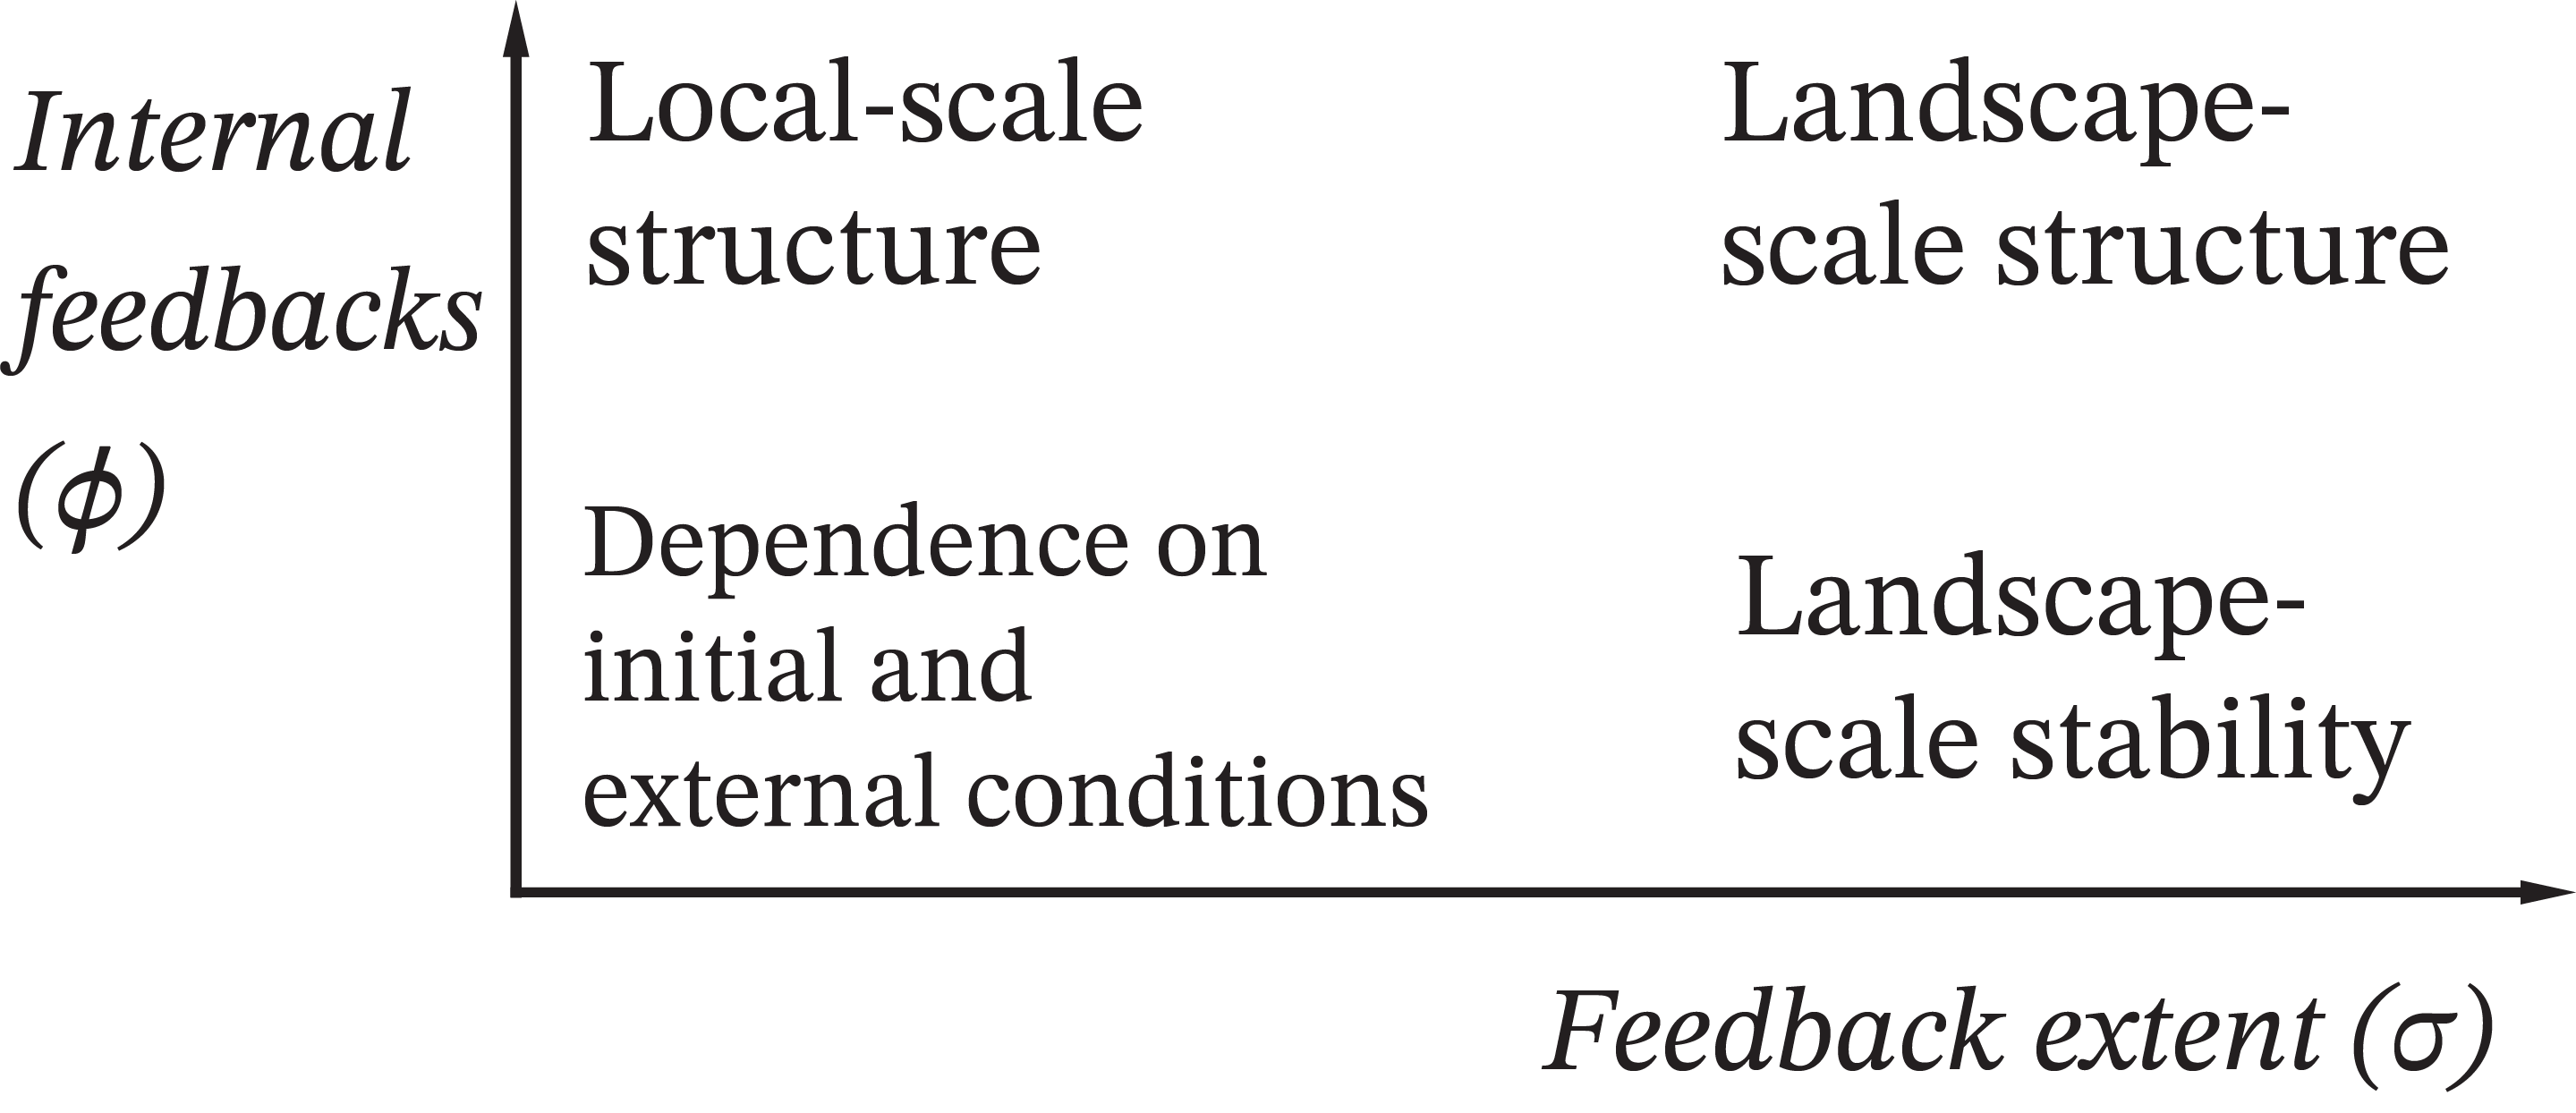
\includegraphics{f1_Change_space.png}
	\end{center}
		\caption{We expect the following dynamics after running the model at varying feedback extents ($\sigma$) and strengths ($\phi$).  At low values of both initial conditions are expected to persist, or changes due to external forcings will be purely dependent on them. In the opposite high-$\sigma$, high-$\phi$ quadrant we expect landscapes to exhibit widespread self-organized structure (with \textit{structure} defined as exhibiting a power-law size distribution.) as internal feedbacks are dominant. At high-$\sigma$, low$\phi$ we expect landscape-wide stability without organization as they are stabilized by long-range feedbacks without strong enough short-range facilitation to lead to structure, and short-range structure without landscape-level effects in the opposite low-$\sigma$, high-$\phi$ corner.}
\end{figure}

\begin{figure}
 	\begin{center}
		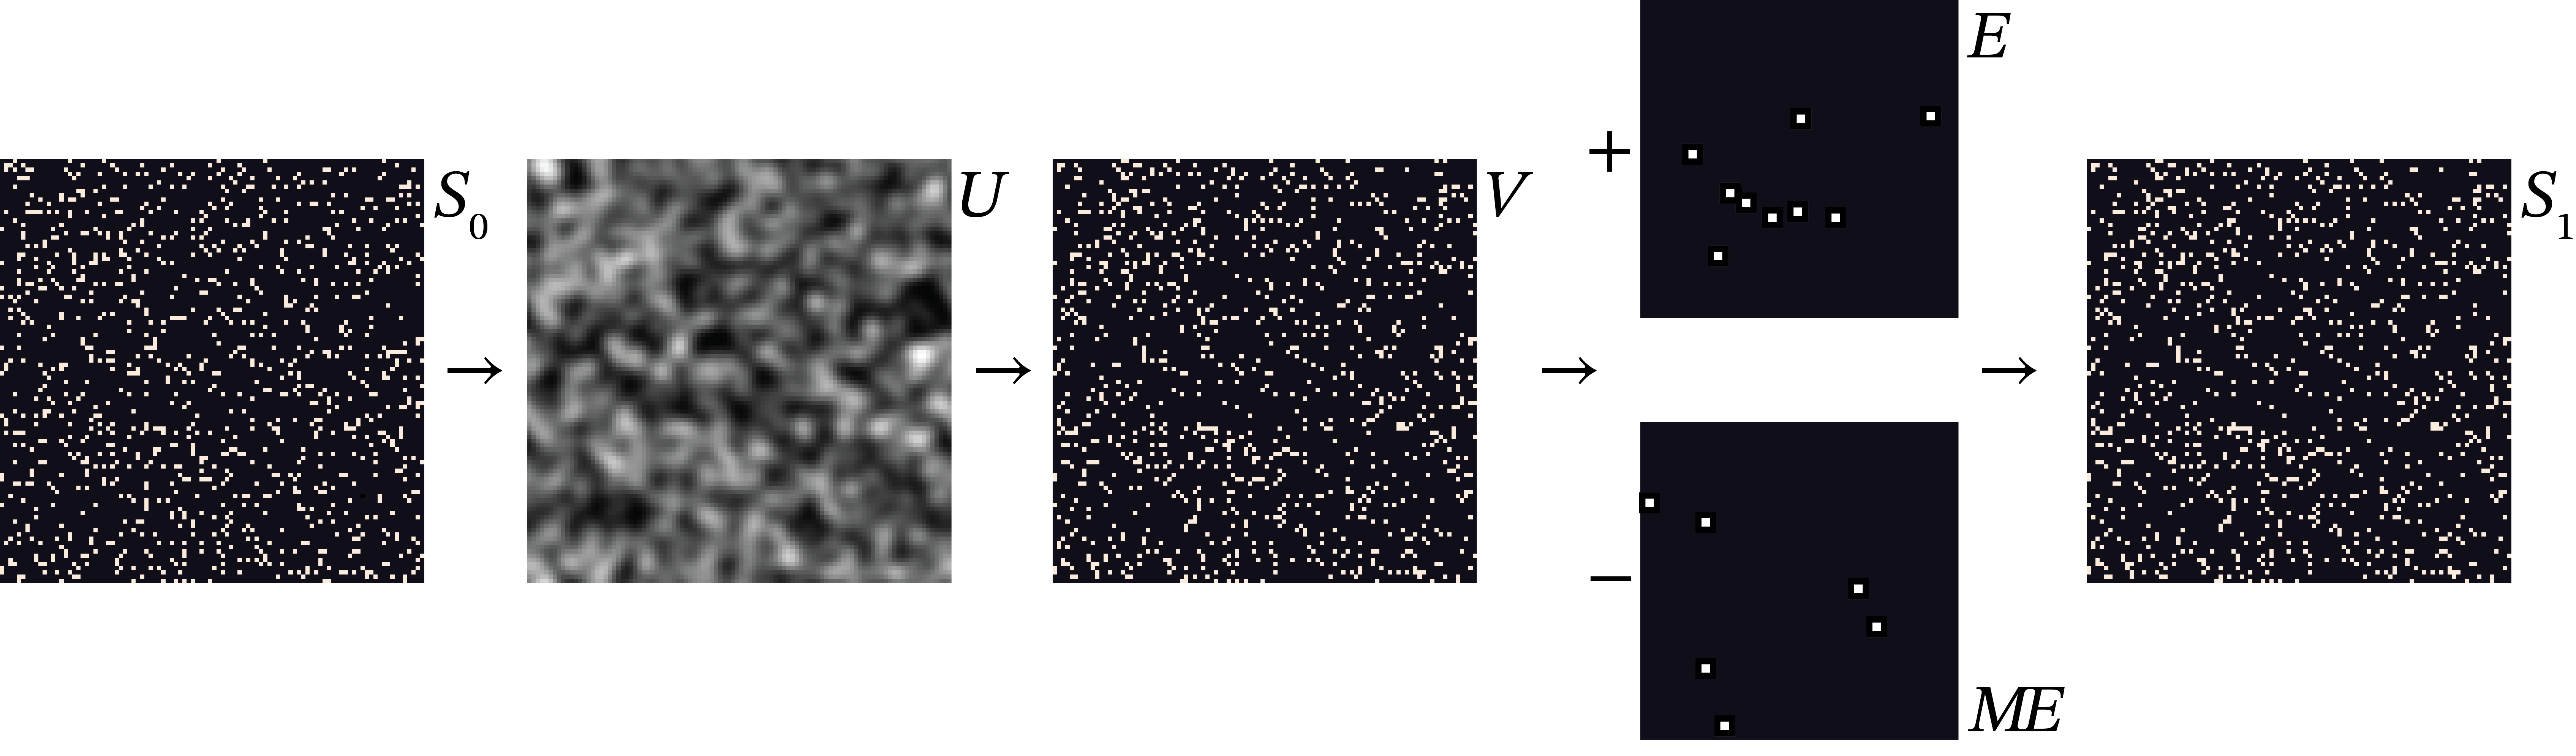
\includegraphics{f2_Model_fig.png}
	\end{center}
		\caption{Diagram of model progression over each timestep: moving from $S_0$ to $U$ we Gaussian blur the initial state grid at a variance $\sigma$. The probability that any given site $x$ on $V$ will be occupied is given by $\phi U_x + (1-\phi)S_x$, resolving into values of 0 or 1. Grids randomly generated for establishment $E$ and mortality $ME$ (with cells magnified here for demonstration) are then added and subtracted, yielding $S_1$. Landscapes depicted are 1\% as large as landscapes used in model.}
\end{figure}


\begin{figure}
 	\begin{center}
		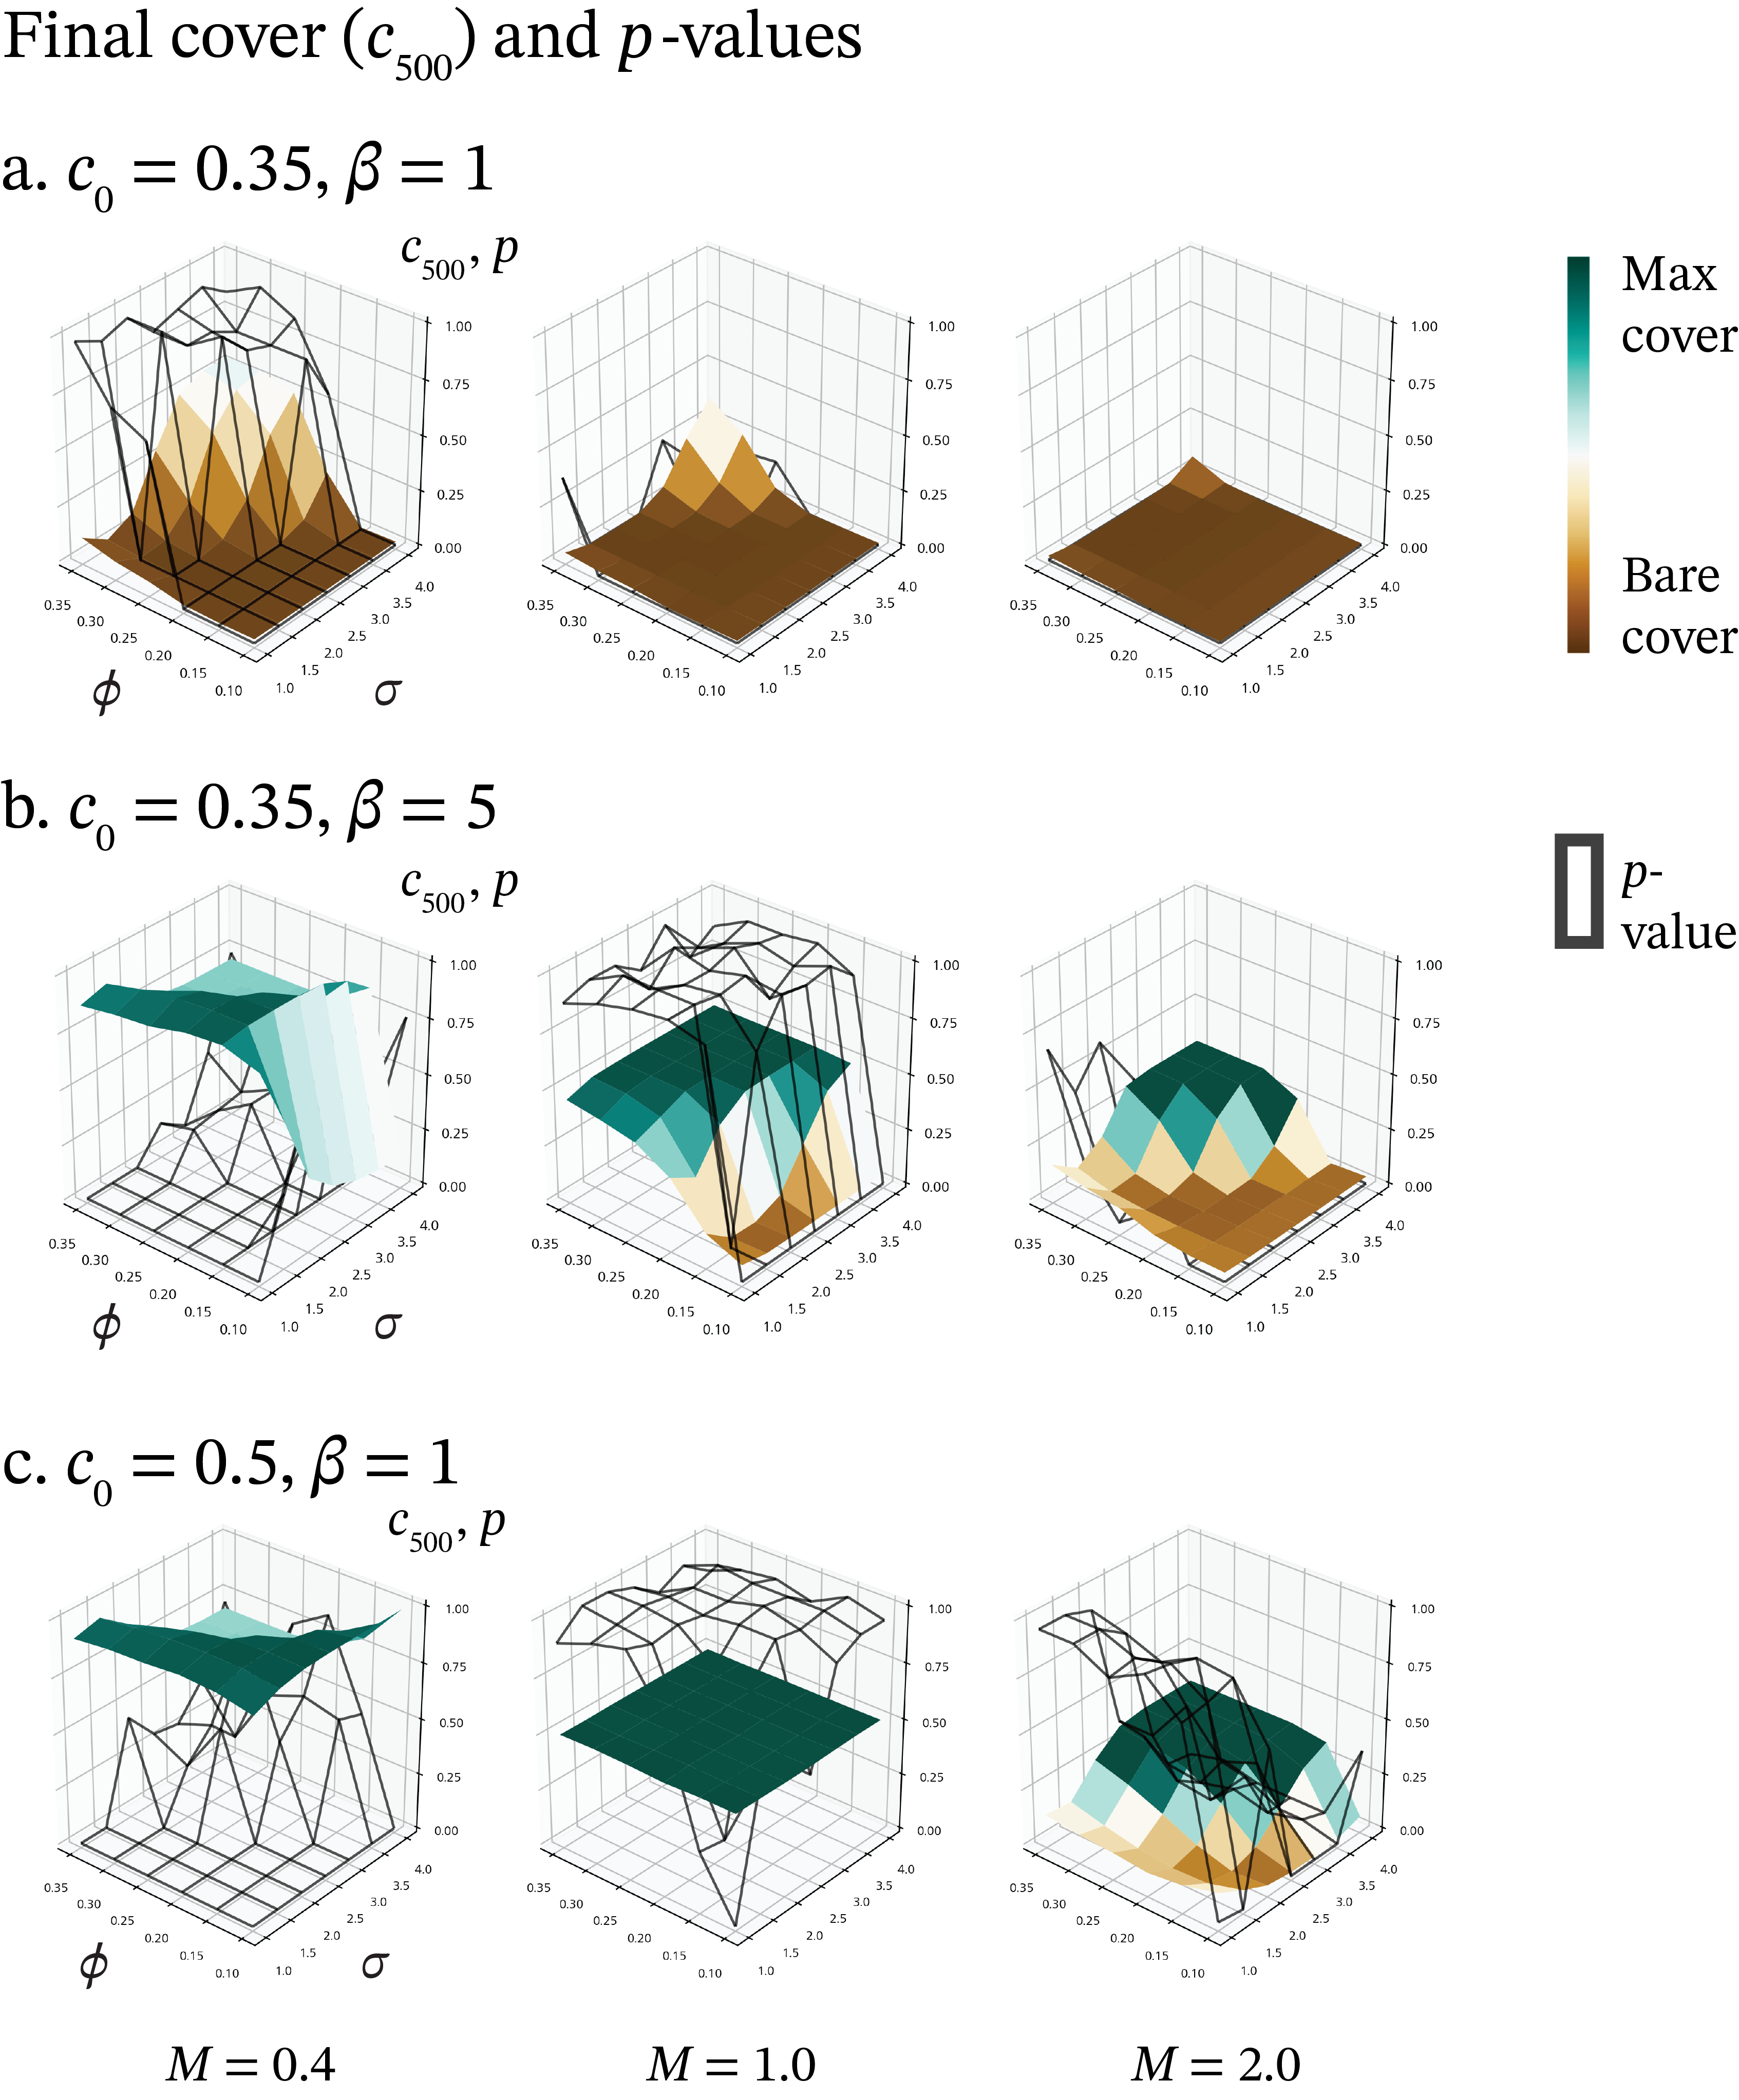
\includegraphics{f3_cover_results.png}
	\end{center}
		\caption{Land cover $c_{500}$ and power law probability $p$ for each $(\sigma,\phi)$ space, with each $(\sigma,\phi)$ surface arranged according to mortality/establishment ratio $M$ and rows based on initial starting population$c_0$ and outside variability $\beta$; row numbering is consistent across figures (e.g. row a. always describes $c_0 = 0.35, \beta = 1$ in figure 4 as well); $c_0 = 0.5, \beta = 5$ is excluded since it has similar cover dynamics as $c_0 = 0.5, \beta = 5$ and the effects of increasing $\beta$ on cluster morphology are similar to $c_0 = 0.35,\beta = 5$ (figure 5). Since cover in the ``high" state is regulated by the overall mortality ratio, the colorbars indicating state are scaled by mortality ratio, not absolute levels of cover. The wireframe surface represents power law probability $p$. Note the special case at $M = 1, c_0 = 0.5, \beta = 1$ where cover is uniform across the ($\sigma,\phi$) surface but power law probability varies.}
\end{figure}

\begin{figure}
 	\begin{center}
		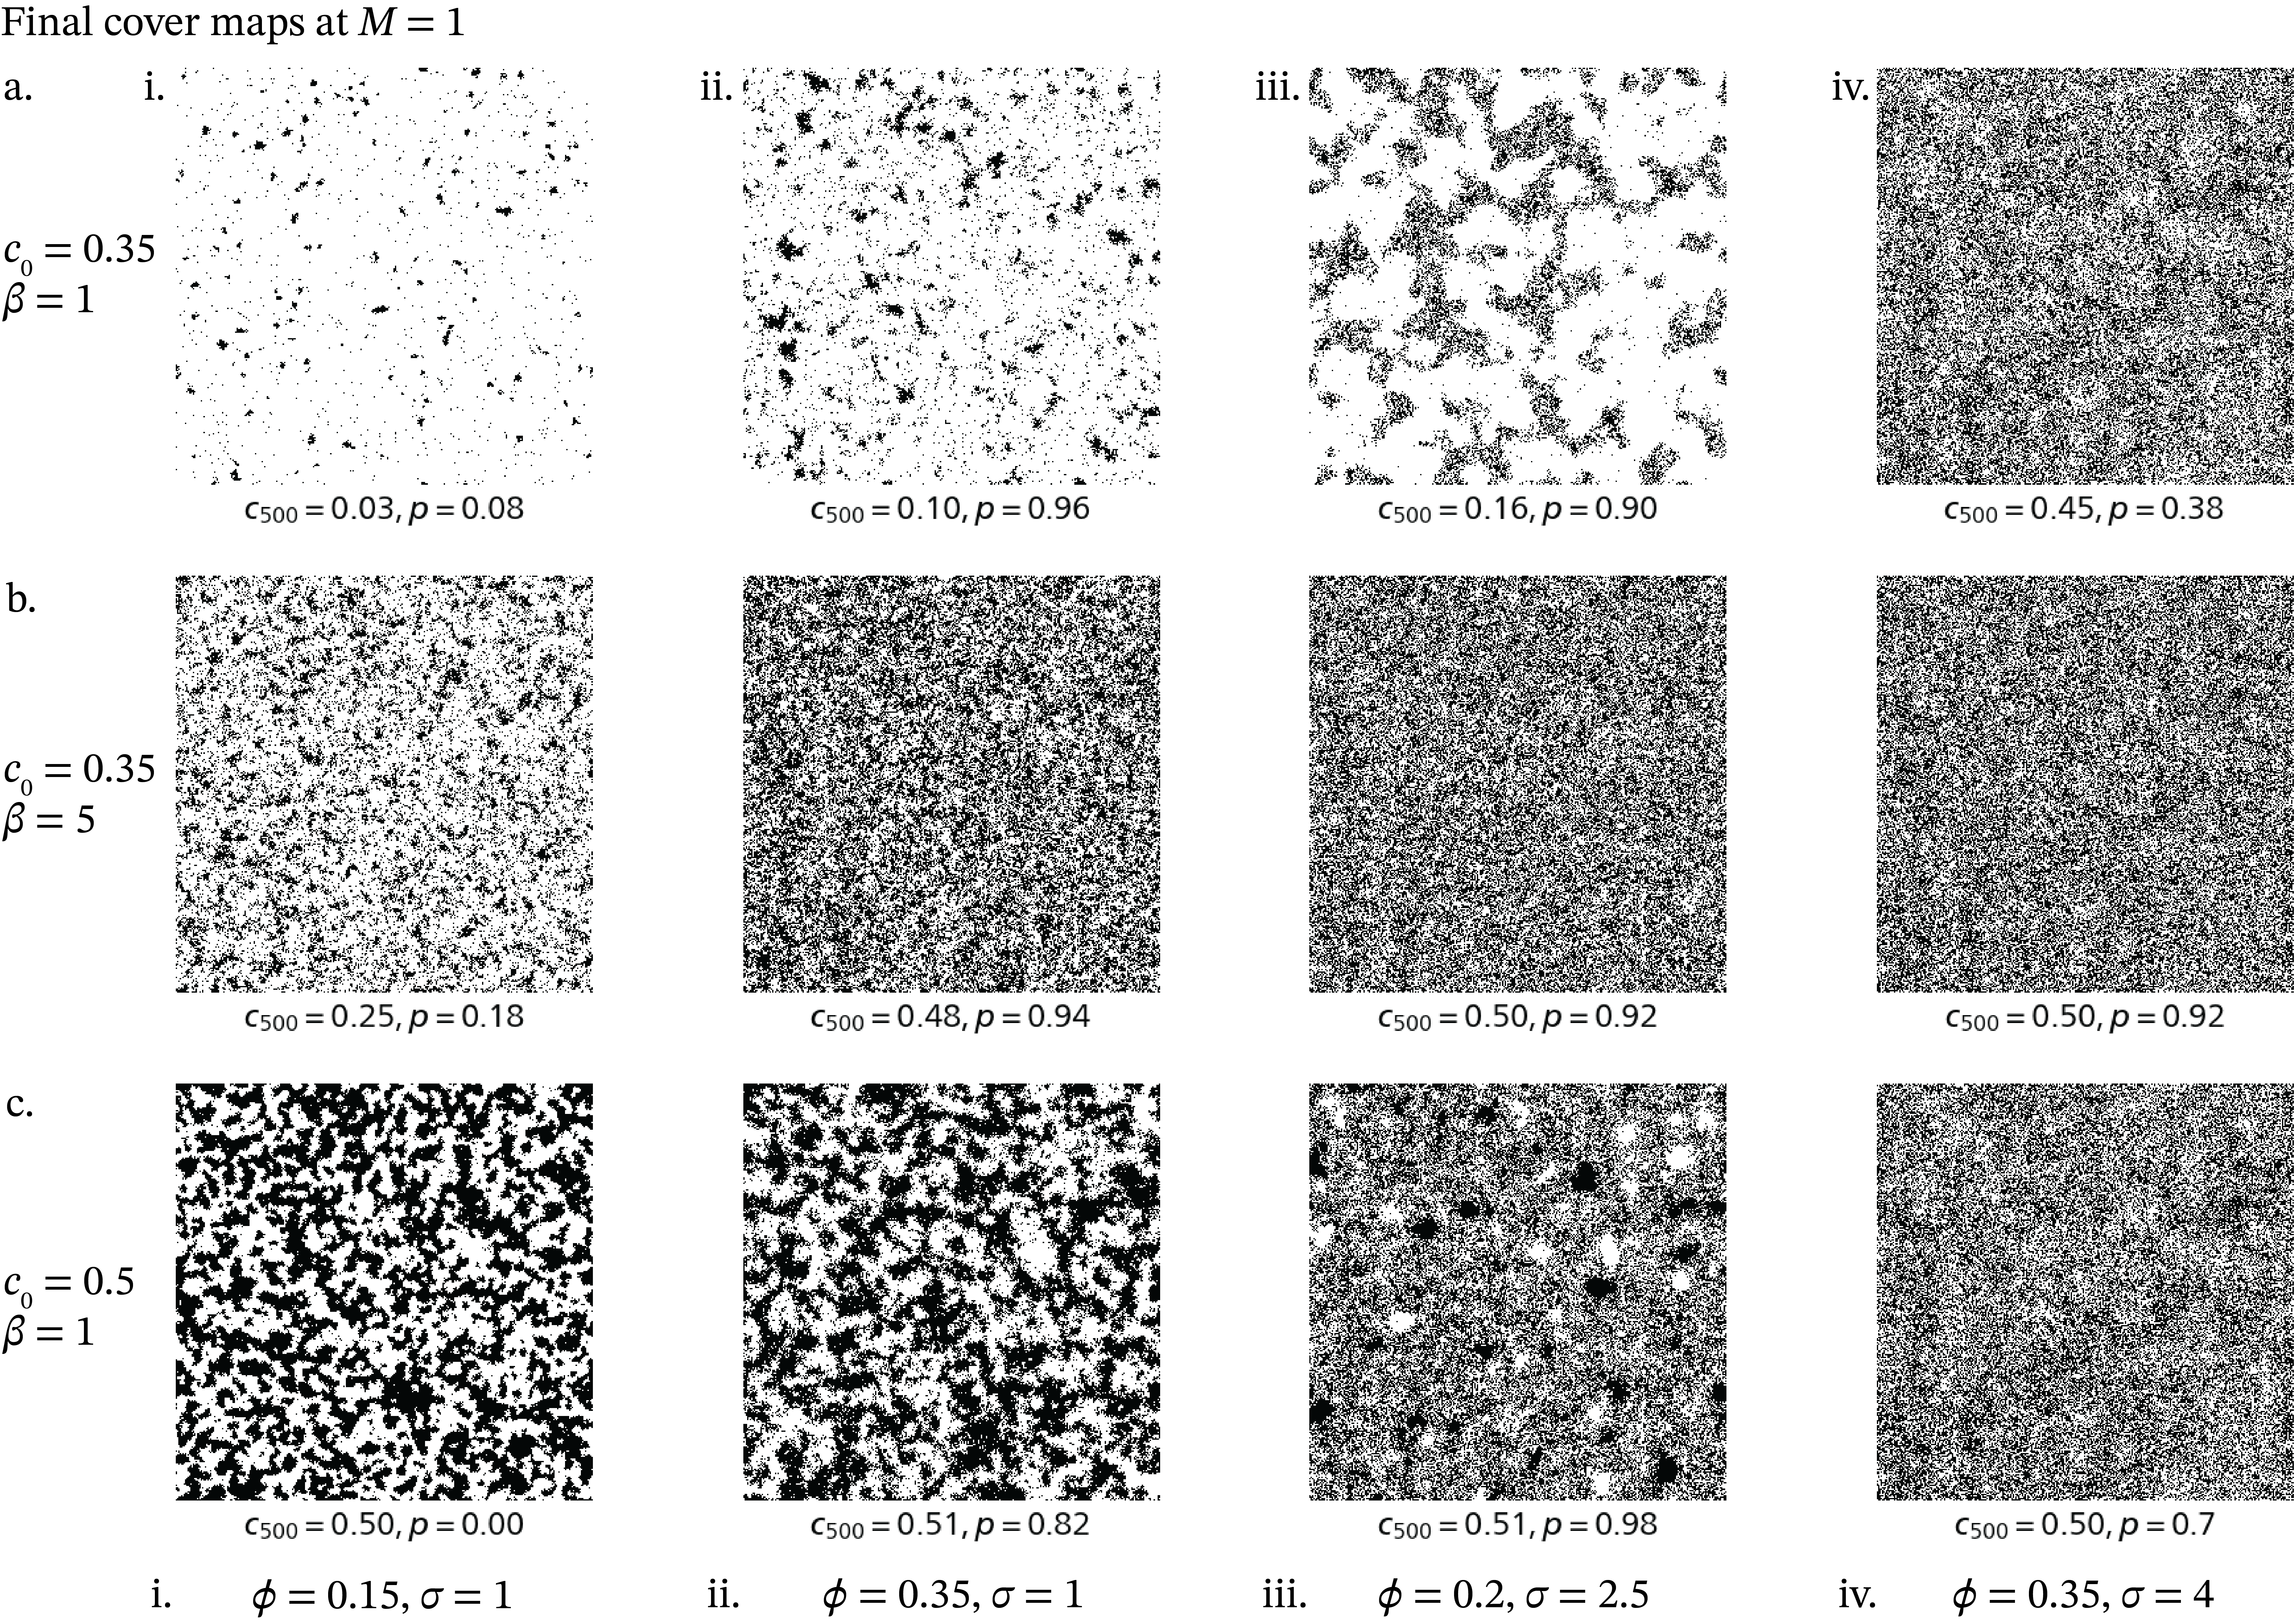
\includegraphics{f4_cartes_trois_niveaux.png}
	\end{center}
		\caption{Examples of land cover $c_{500}$ at $M = 1$ Column i. is the low state at minimal $(\sigma,\phi)$. ii. is the intermediate state and minimal $\sigma$, maximal $\phi$, iii. an unstable at $t = {500}$ state at $(\sigma,\phi)$ = 2.5,0.2, declining to the low state in row a., increasing to the high state in row b, and in a steady state of cover row c., and column iv. is the high state at maximal $(\sigma,\phi)$.}
\end{figure}

\begin{figure}
 	\begin{center}
		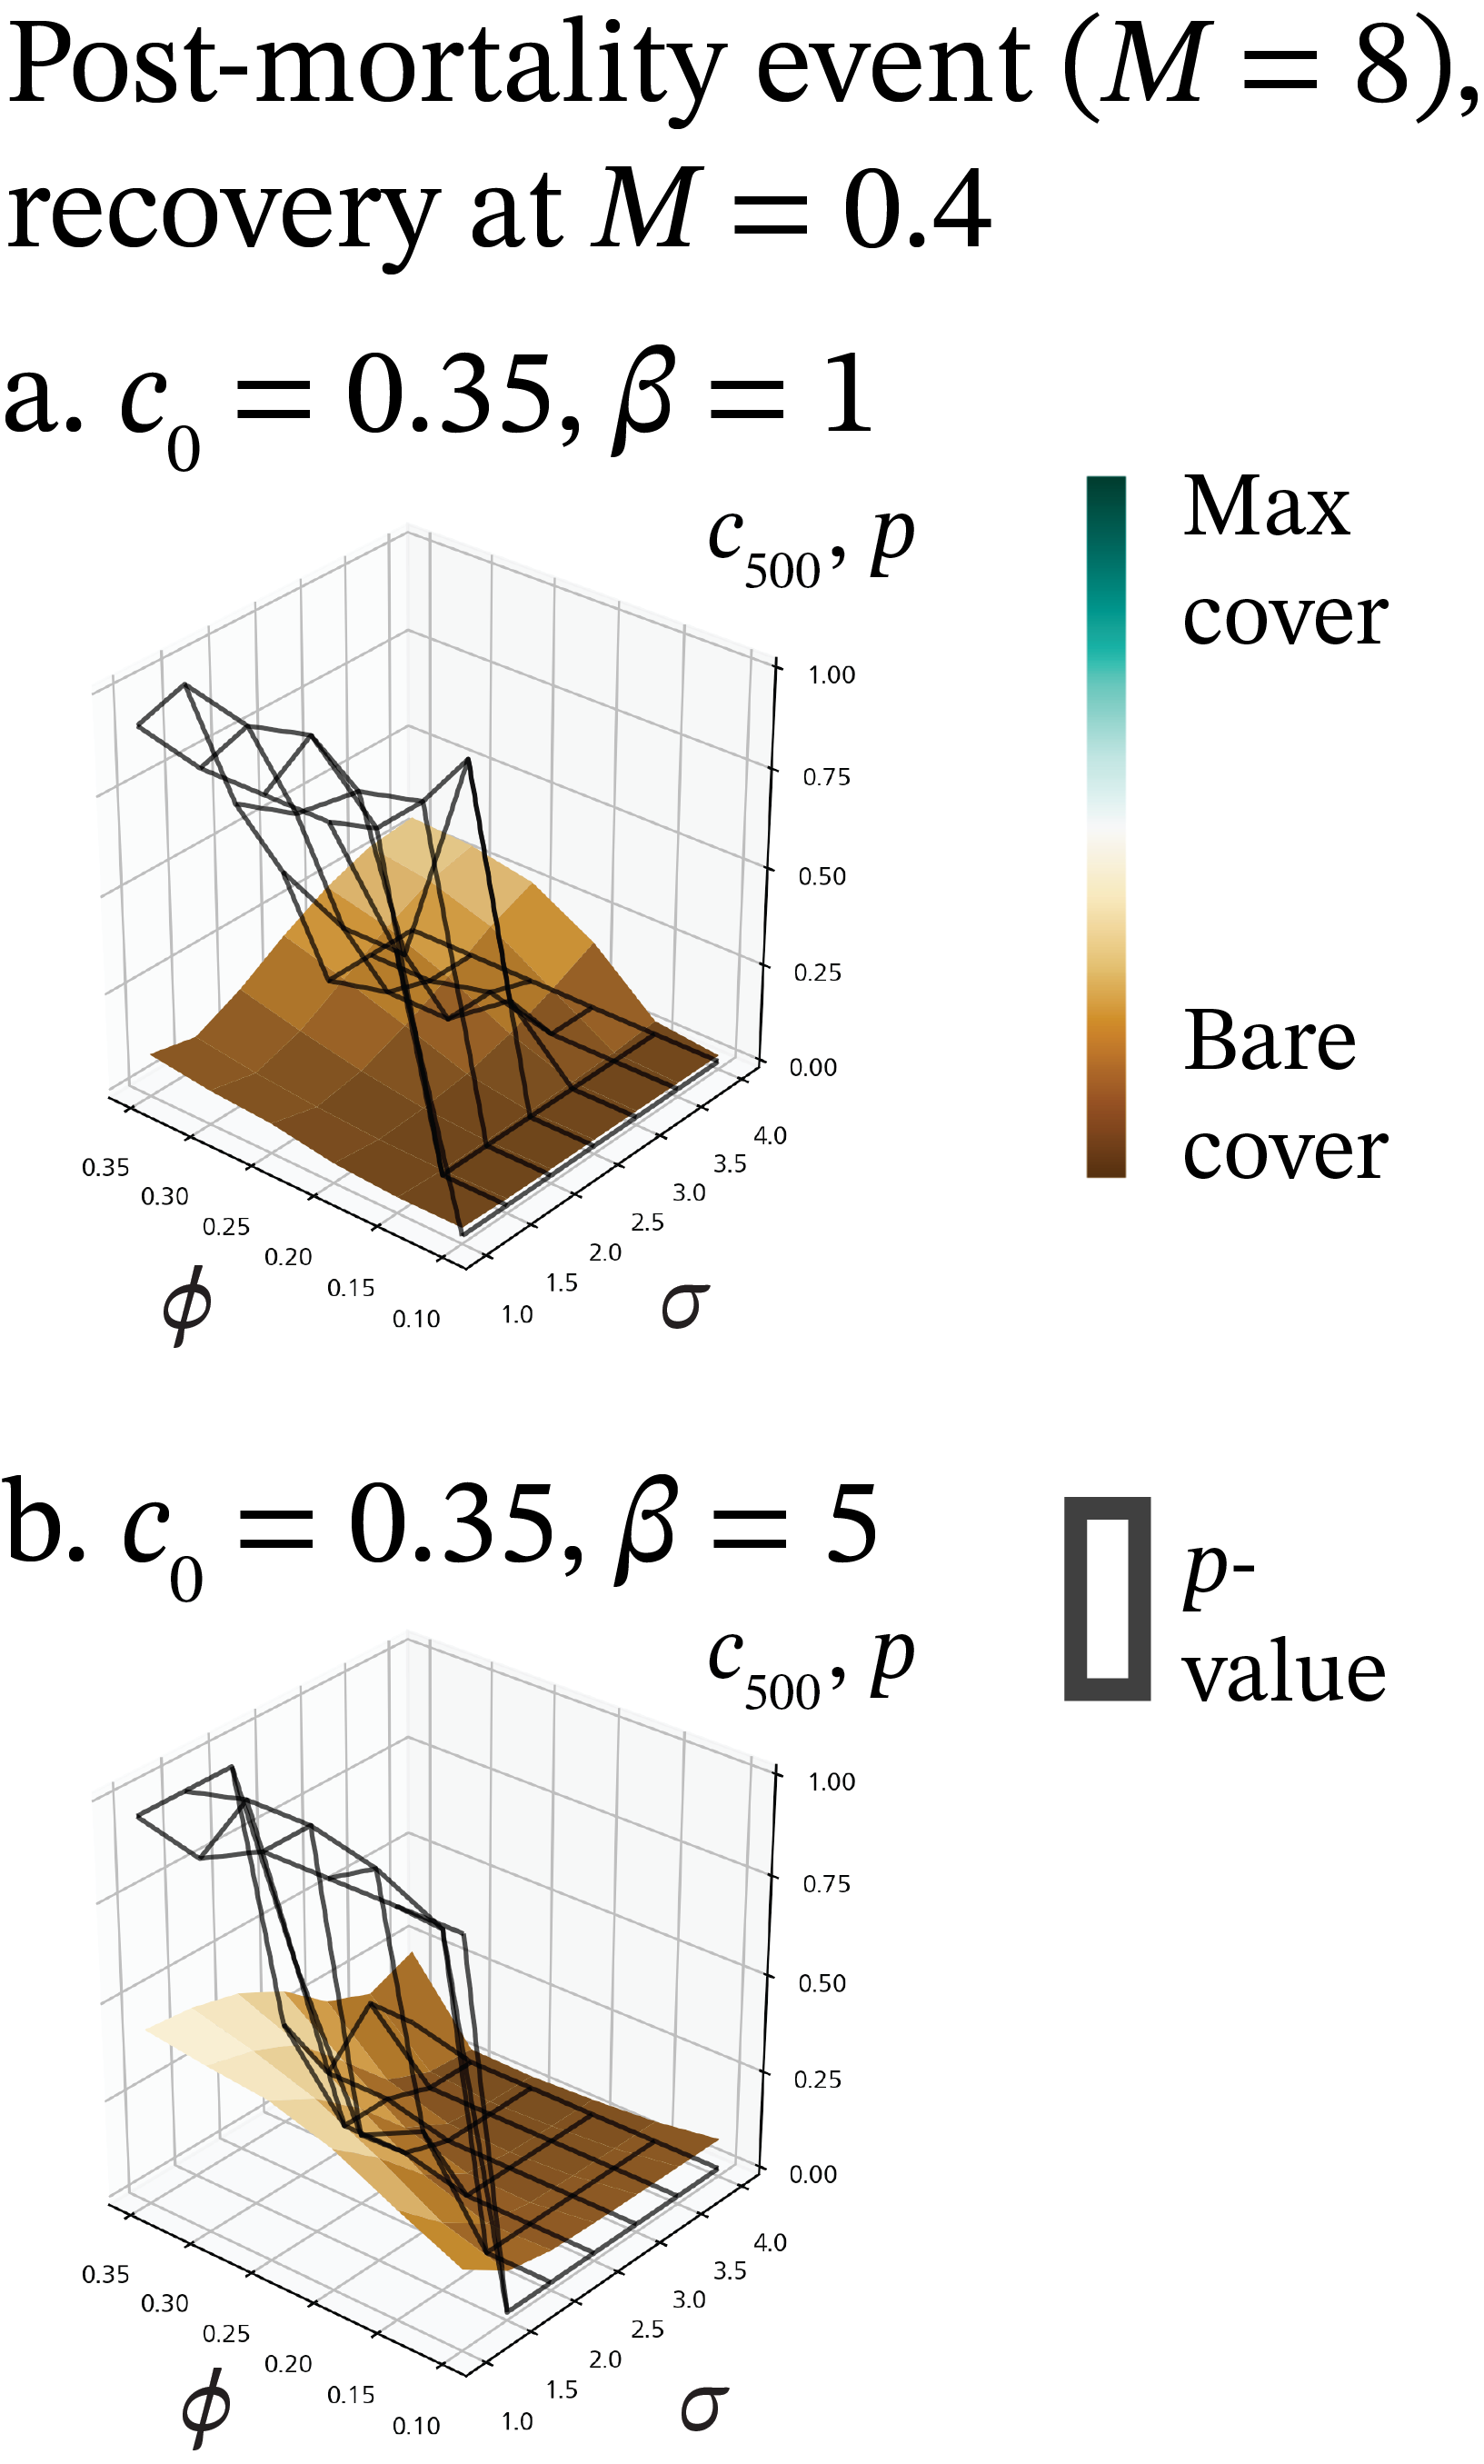
\includegraphics{f5_cover_results_dist.png}
	\end{center}
		\caption{$(\sigma,\phi)$ surfaces for land cover $c_{500}$ after a mortality event at $M = 8$ and a recovery condition of $M = 0.4$ for greater clarity of recovery dynamics; similar dynamics are seen at $M = 1$ and $c_0 = 0.5$ and are excluded for conciseness, as are cases when $M > 1$ as they exhibit zero recovery after the mortality event.}
\end{figure}

\begin{figure}
 	\begin{center}
		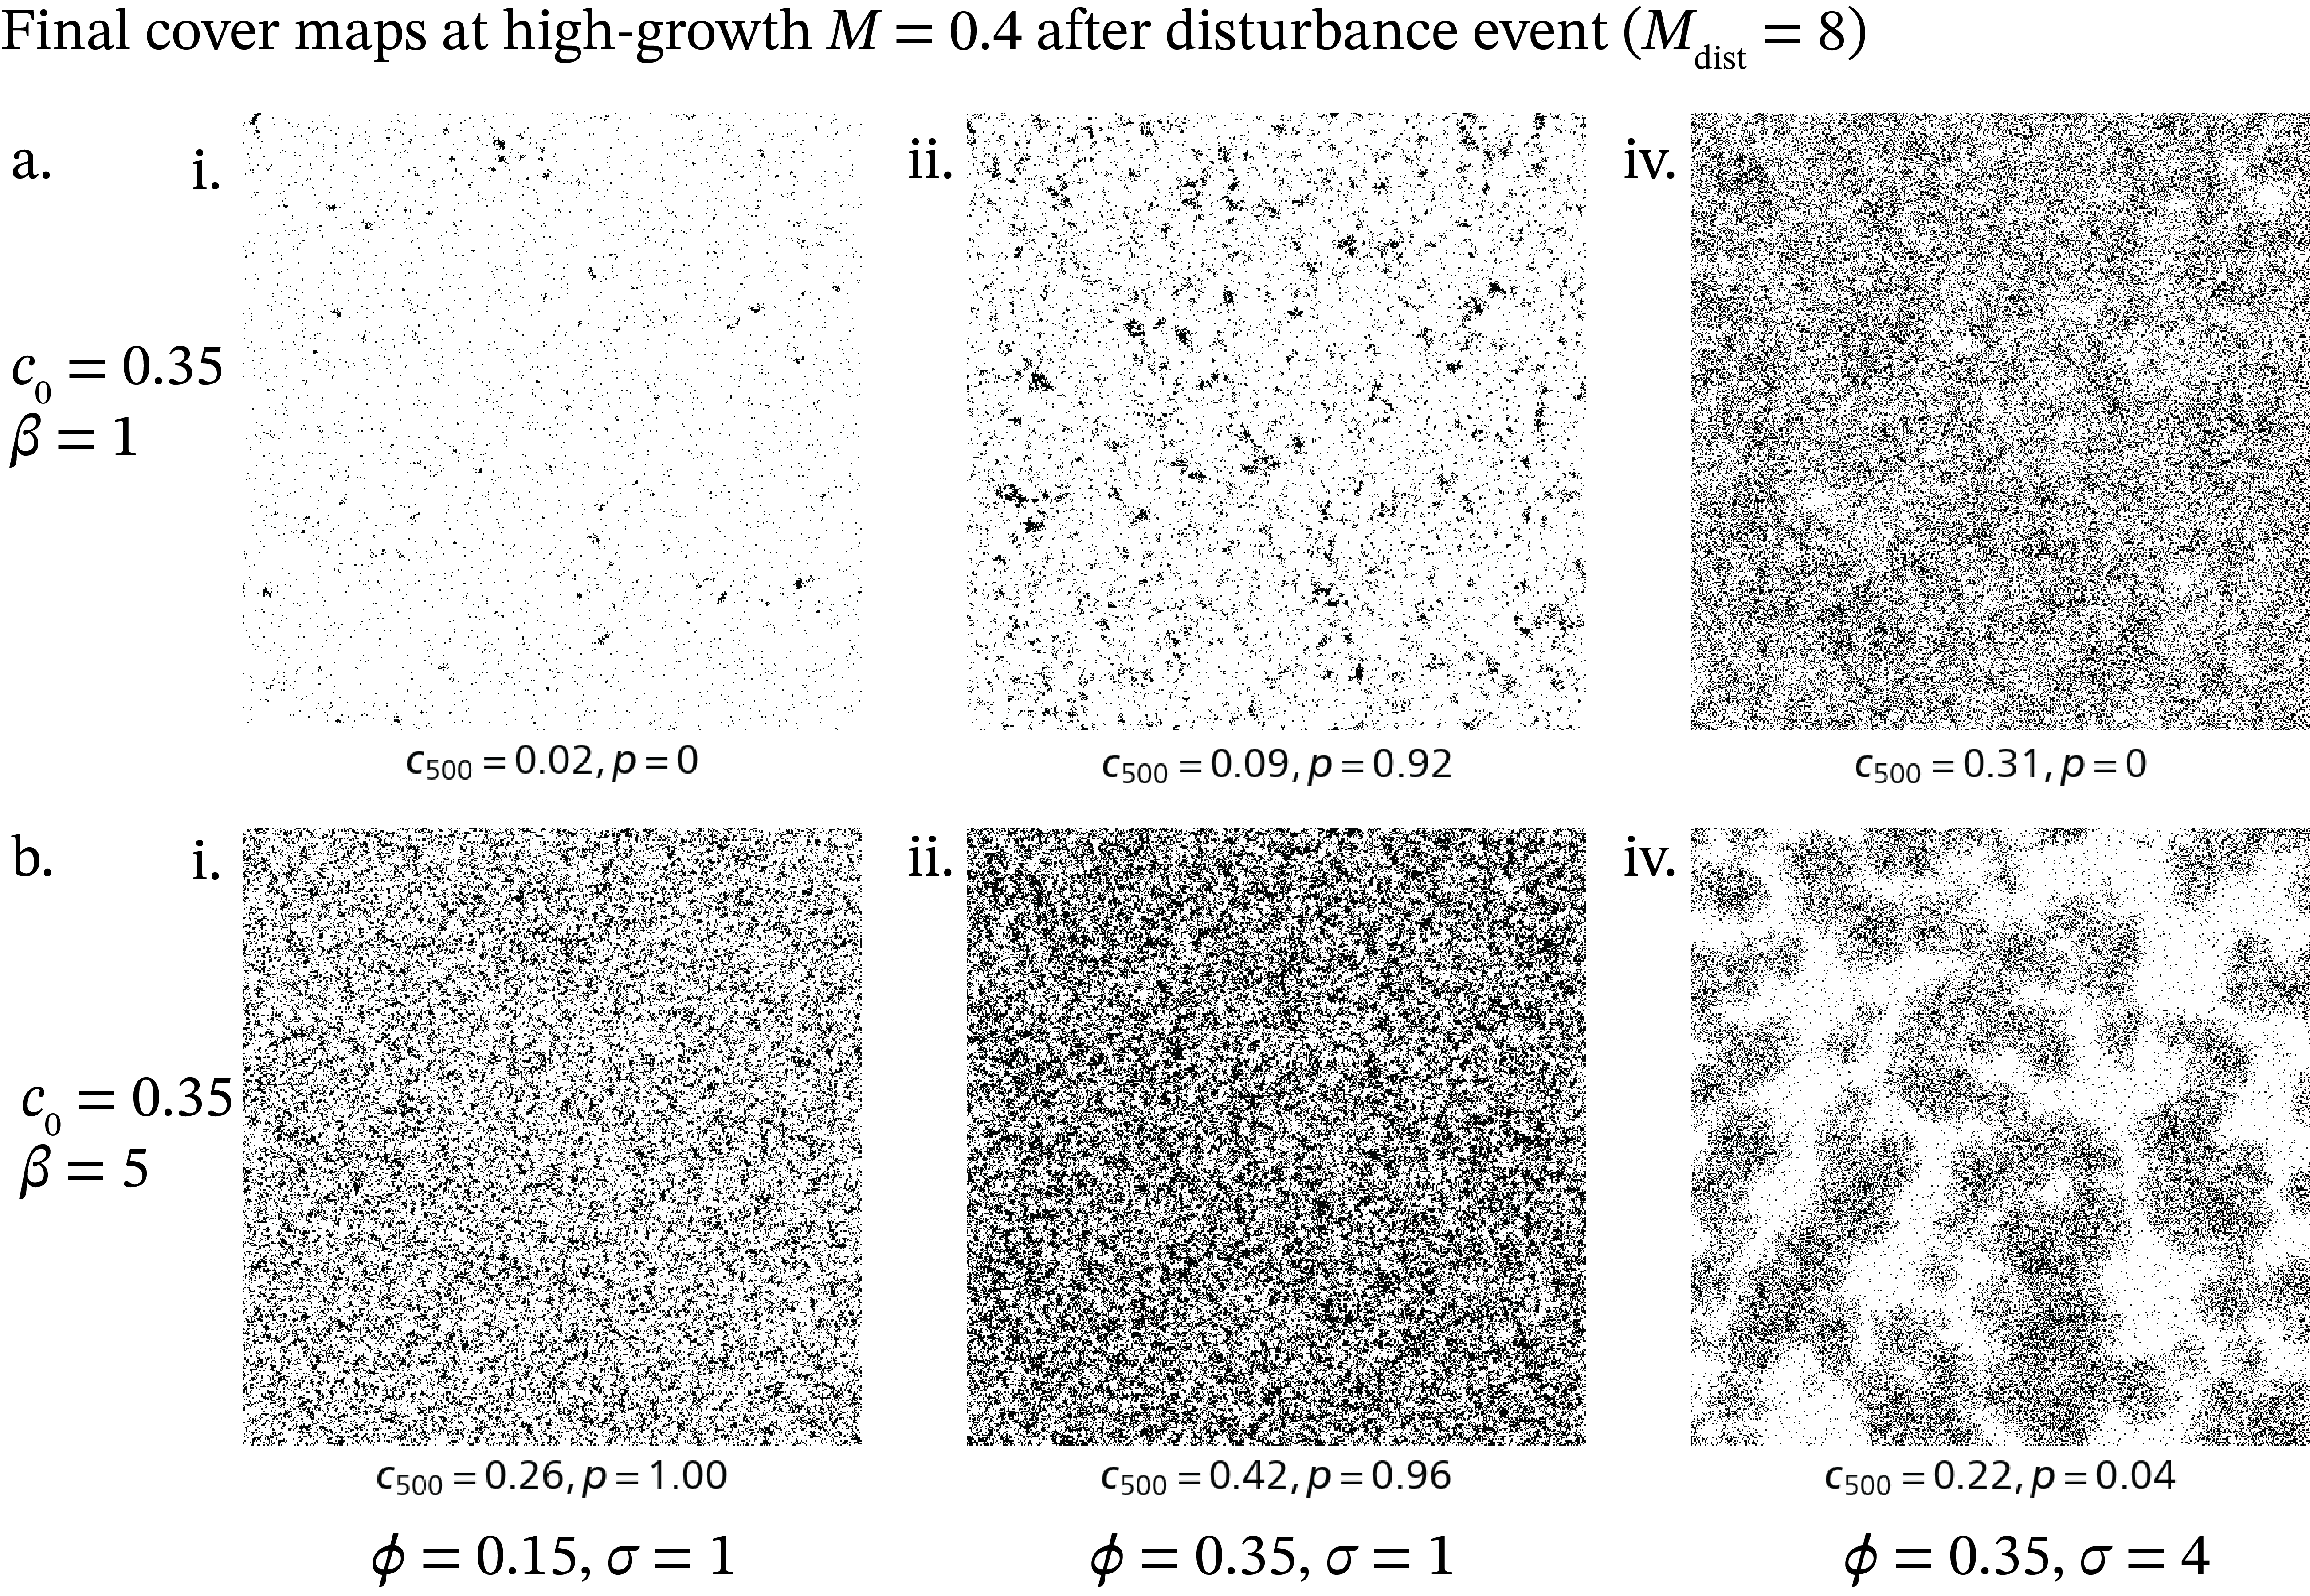
\includegraphics{f6_cartes.png}
	\end{center}
		\caption{Examples of recovering land cover $c_{500}$ on the $(\sigma,\phi)$ surface after a mortality event at $M = 8$ and a recovery condition of $M = 0.4$ for greater clarity of recovery dynamics. Examples from the middle of the surface ($(\sigma,\phi) = 0.25,2.0$) are less relevant so column iii. is excluded.}
\end{figure}

\begin{figure}
 	\begin{center}
		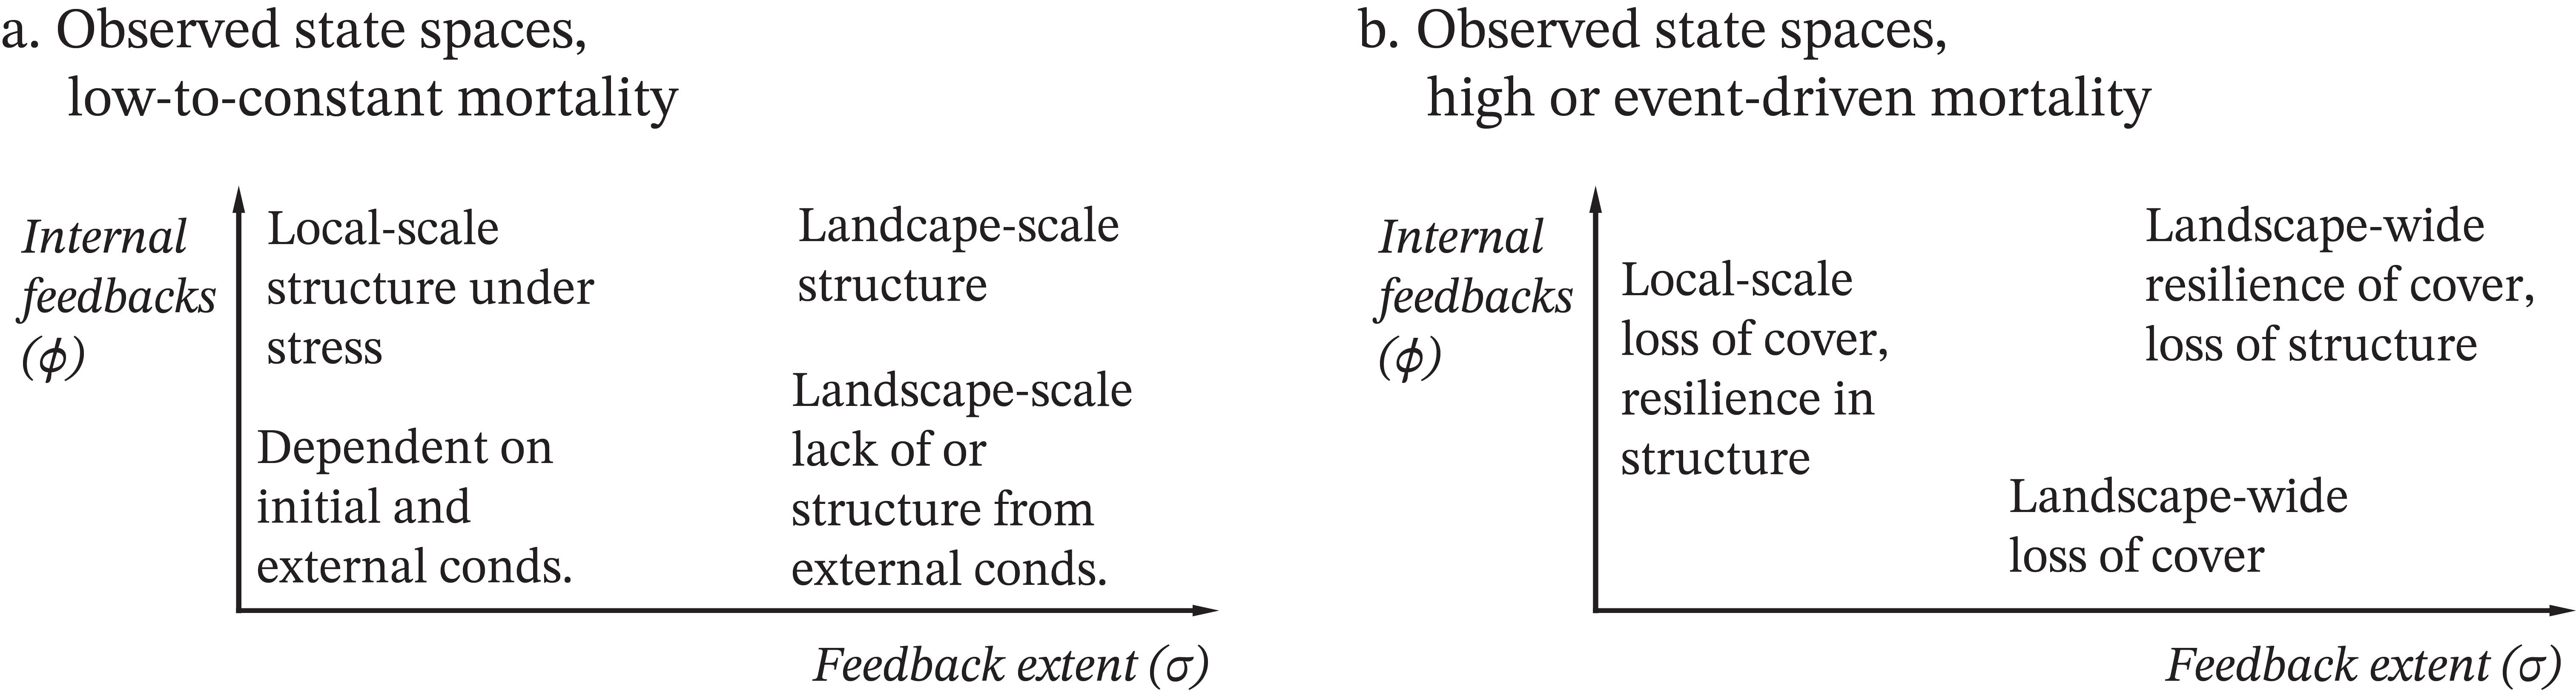
\includegraphics{f7_post-experiment.png}
	\end{center}
		\caption{Revising the expected change space in figure 1, in diagram a. we find a broad similarity with expectations from figure 1 with some revisions. Only the minimal and maximal corners in $(\sigma,\phi)$ space consistently manifest. The high $\sigma$, low $\phi$ corner can take on the characteristics of either the minimal or maximal corner depending on starting population and outside conditions, with a greater tendency toward the unstructured state. The low-$\sigma$, high-$\phi$ corner only manifests a distinct set of local-scale dynamics under stress, but converging towards the unstructured state when $M < 1$ (figure 3). Under greater stress or after a mortality event the dynamics in structure and cover are often reversed, with some cover remaining at the maximal $(\sigma,\phi)$ corner without structure but stronger resilience or growth of locally self-organized cells in the higher-$\phi$ area, which lead the recovery of the landscape (figure 5)}
\end{figure}






%Under conditions of stress this structure can be broken, and under extreme stress the breaking of connectivity leads to the presence of hard boundaries between the heterogeneous and gap state as long-range connectivity is broken. Strong short-range connectivity allows as a means of resisting such overall loss of structure (even as cover is reduced) since such short-range incorporation of interannual noise is ``protected" from widespread mortality. Such systems may be termed robustly critical due to their survival over a wide parameter space. The breaking of long-range connectivity, then, has implications 
%
%More on the spatial aspects of criticality.
%
%
%At high levels of external noise the system's transition is mainly what one would expect---going from lower to higher interannual noise $\beta$ (best illustrated by figure 3a-1.0 to 3b-1.0 and 4a-i to 4b-i) at short feedback ranges even small clusters without a power law exhibit the sort of shift expected from literature, with power-law relations between clusters as state changes. Final states under weak, inextensive feedbacks can still exhibit heterogeneity, though without power law structure. However, states characterized by more extensive or stronger feedbacks this power law structure is maintained even after landscape transition as interannual noise is processed by spatial feedbacks, either well-mixed, landscape-wide, relationships by networks of clusters or poorly-mixed, isolated clusters in cases of spatially inextensive but strong feedbacks. While, in the parameter space, there were strong thresholds between the final development of a low or high state, there is little evidence of thresholds in transition from the initial random state to the final state, consistent with observations of undisturbed ecological systems. However, relatively-hard edged spatial between a high, well-mixed state with high power-law probability and a low state in cases where connectivity is either relatively short or disrupted.
%
%While at large degrees of aspatial noise result in total, landscape-wide shift to a high or, in a limited area at or centered at the low state centered at the $(\sigma,\phi) = 1.0,0.1$ (note that $\beta$ in figures 3a,b-1.0, 4a-i,b-i the cell or cells centered at or near the low-feedback attractor are at or approaching low cover), accelerating landscape-wide transitions (e.g. 4b-iii), at low levels of noise we can see this transition still in progress as in figures 4a,c-iii, with 4a-iii reducing retreating from higher initial cover and state and 4c-iii in a steady state with both high and low areas. Rather than the retreating or expanding clusters, there is a retreating or expanding clusters seen at low spatial extents, we observe not expanding or retreating clusters of intermediate size but expanding or retreating \textit{areas} at the high state. This combines the mortality-recovery dynamics of mature landscapes with the spatially-organized, but based more on local or cluster-edge spatial dependence than self-organization, with areas of high and low state existing simultaneously. While the search for and examination of dynamics over large temporal and spatial gradients is an area for further investigation, this pattern also bears some relation to the disturbance of a landscape's high-state, breaking their extent and providing an area for an alternate or bare state to develop and expand (as in deforestation in tropical forests; CITE). In this model considering such a disturbance-driven change in feedback extent would be represented by shifting from one cell of the $\sigma,\phi$ surface to another or comparing with equivalent coordinates on the corresponding the hysteresis surfaces rather than applying different conditions in different spaces, having feedback extent and strength shift dynamically based on gap and vegetation, and including a different set of responses to $M,\sigma,\phi$ for each type of cover. 


%SHIFT ON GLOBAL SCALE. WHEN FEEDBACKS ARE STRONG BUT LOCALIZED SOMETHING LIKE ROBUST CRITICALITY. FURTHERMORE, BOTH CRITICALITIES MIX DURING LANDSCAPE EXTENSION, AS . EMPIRICAL REPRODUCTION OF ABOVE STATES, BUT A SLOWLY GROWING OR RETREAting high state?
%
%COMPLETE ANISITROPY. best evidence comes from 
%
%While changes in landscape tend to exhibit power-law relationships. As the amount of stochastic noise increases even clusters in the non-power law, even in our resilient, non-power law area evidence of a power law begins to be exhibit, providing evidence of an incipient landscape shift. At 
%
%Different external conditions leading to different attractors depending on outside conditions. Enough stochastic noise will force state change. 
%
%Convergence towards attractors based on combined effects of ($M, \sigma, \phi$), with minimal variance in levels of cover apart from transitional stages, only different distributions of cover. Domino effects from random perturbation. Have to reread KIZASHI. Persists across parameter space. Short vs. large, uniform heterogeneity.  Exhibits critical dynamics at multiple scales: across the landscape, with clusters dying out as larger ones expand, within clusters given spatially-dependent expansion. 
%
%: obvious low state lack of pattern. Shift to scale-free dynamics lead to spread across landscape over time, passing a critical phase as full high-state approached, but within expanding regions as still regulated by overall mortality and recovery dynamics, even as expanding. Both cover and structure sensitive to perturbation but not the Exhibits well-mixed and robust criticality at once. Little evidence of self-organized criticality in the sense of change. 
%
%No vectors of change---for instance distribution in a preferred direction.
%
%While this paper demonstrates that, while power law structures do have implications in detecting landscape change generated by spatial feedbacks, they nonetheless are not dispositive evidence of transitory states between landscape changes. Although the entire parameter space tested had some degree of spatial facilitation it does not necessarily hold for the creation of the characteristic patterns in landscapes. While short-range facilitation can be overwhelmed by external establishment or mortality (figure 3a,b,c-0.4,2.0), in cases of less extreme outside variability initial conditions play a larger role. With high cover this results in a relatively hard-edged mosaic as short term facilitation organizes landscapes into fairly homogenous vegetated and gap spaces: strongly patterned as a result of spatial feedbacks, but not \textit{structured} by power law relations among patch sizes. At lower initial vegetation levels this results in localized areas of resistance, but with a size distribution weighted towards larger patches.
%
%Where power-law relations do exist---and they can exhibit similar broad-scale patterns as the cases noted above, just with a noisier edge---they can indicate transitional, stable, intermediate, and recovering landscapes depending on broader conditions. As such, while power law distributions can be evidence of landscape structure, since power law feedbacks, while found in areas in our model with incomplete spin-up, can also be found in certain stabler states. Depending on the extent and strength of feedbacks, different scales of pattern are also possible, even as power law likelihood and overall land cover remain similar (figures 4c-ii., 4c-iii.). TOGETHER, THESE ARE ALL CONSISTENT WITH AMBIGUOUS RESULTS NOTED ABOVE. POWER LAWS CAN BE SIGNALS OF STABILITY
%
%IDENTIFY THE PRESENCE OF THRESHOLDS OF VARIABILITY NOT JUST DETERMINED BY NOISE, BUT BY THRESHOLDS IN LANDSCAPE PROCESS OR LANDSCAPE VARIABILITY. 




%While most attention has been paid to combined short-range facilitation, long-range competition models of landscape dynamics (see \citet{Borgogno2009} for a comprehensive review of these methods), it is worth noting that gap follow the same dynamics as vegetation, with the facilitation for vegetation competing with the facilitation reinforcing gap spaces at the expense of both initial and new vegetation.

%with the low state, high establishment, particularly with interannual variability increases, quickly overwhelms any spatial facilitation and structure, with the intermediate/metastable state only appearing at higher $M \ge 1$ and  Typical candidates for the sort of coarse spatial heterogeneity here are ecohydrological. Given the facilitation over distances root area effects facilitating infiltration are particularly attractive, though under-canopy effects such as shading or preventing rainsplash compaction of soil surface are possible as well (though see below, \citealt{DOdorico2007,DOdorico2005,Scanlon2007,Bhark2003,Wainwright2009}). Have some nearby extent. 

%Strong but somewhat more diffuse,

%Nonlocality, even at a small degree, determines this. Any sufficiently diffuse feedback will converge on aspatial change. 

%Isometry of change: in all cases we have isometric change, either around our cells or from without



%In figure 4c-iii cluster size distribution does follow a power law relationship, they are not spread evenly across the landscape but are included within larger connected or near-connected ``megacluster." The power law distribution comes from uniform heterogeneity within this larger, shrinking, megacluster. This porous megacluster contrasts with

%Another weakness is that we cannot

%

%Shift towards

%Such spatial, but hard-to-scale processes are likely not associated with any one feedback but rather a cluster of related facilitative effects, e.g. intra-cluster interspecific facilitation as suggested in MAESTRE or very localized under-canopy hydrological or nutrient (via recycling of lead litter DEBRIS) feedbacks. Since such feedbacks are related to adjacency or near adjacency of plant parts, such as canopies or root zones, scale would be species-dependent, on the scale of meters or less.

%It also corresponds with the observed threshold behavior between a largely-empty and largely-occupied spaces. However, these landscape-scale states, while largely homogenous at the landscape level, can exhibit local heterogeneity. This is particularly true of the higher-$\phi$, higher-$\sigma$ cases: often the zone of higher land cover is highly heterogeneous thanks to the harvesting effect of random mortality. Where $\phi$ and $\sigma$ are at their maxima in such cases the role of facilitation plays in rearranging growth is as significant as its role in fostering or maintaining it. Thus while there may be a classically critical transition between largely empty landscapes and fuller landscapes, \textit{within} that fuller zone there is something analogous to robust criticality, where there is little evidence of strong thresholds, only convergence towards a state determined by the relationship between $\beta$ and $M$ limited by landscape-wide feedbacks. 

%While the above model does not provide a mechanistic explanation for landscape heterogeneity, the variety of results described above do correspond with observed heterogeneity in landscapes, and thus can provide insightsinto the role of process scale in processes larger-scale changes into finer-scale shifts in vegetation. In the context of figures 3 and 5, this section deals not with shifts across a single subplot but rather shifts between subplots, as external conditions change specific mortality rates and become more-or-less variable per cycle.




%
%
%To move from this area of low power law probability to the intermediate, metastable state requires more robust feedbacks, able to operate as increasing interannual variability drives up chances of mortality. Again canopy or root-zone processes are likely to be 



%Furthermore, t is also worth remarking that there is little 
%
% Such facilitation requires \textit{adjacency} to operate, such as the under-canopy recycling of leaf litter or canopy or patch-area shading \citep{Zeng2004} WANGHESS? OTHERS. 

%While it is important to remember each case in figures 3 and 5 represents a parameter space, paths to landscape change can be thought of as moving a point across each parameter space to reflect changing internal spatial structures or, crossing subplots, changing interannual outside inputs. This is not sufficient to provide a mechanistic explanation for processes driving feedback growth, rather pointing towards potential signals in structure or cover in identifying landscape state and change. 

%These effects are more ambiguous than implied in previous models, but can still help situate those previous results in different cases of landscape change and stability.





%However, such cases only occur when there is a relatively stable ratio of mortality to establishment, and even in case 4a-i the overall cover level is much less than in the initial condition since at $t_0$ gap area was larger than covered area, giving gaps an initial advantage in overall spread---initial conditions determine the final one. As the establishment/mortality ratio diverges from one, either case becomes dominant across the landscape with minimal organization as random establishment or mortality events on each cell are minimally influenced by nearby ones. Even if landscape maintenance relies on very-close-scale feedbacks, landscape change depends largely on outside influences.




%There are two routes to the high state---one via increasing spatial feedbacks
%
%Either of the above mechanisms proves resilient over 
%
%
%Key t
%
%
%Such an effect could thus be in the ``high state" of relatively extensive and strong feedbacks, and unlike many hydraulic models is a simple process with strong empirical support. 
%
%ALTERNATIVE 
%
%While most attention has been paid to combined short-range facilitation, long-range competition models of landscape dynamics (see \citet{Borgogno2009} for a comprehensive review of these methods), it is worth noting that in this purely facilitative model spatial feedbacks still results in landscape heterogeneity exhibiting power-law likelihood, as random 
%
%This explains why the ``high" state in 3b,c-0.4 is actually \textit{lower} that than the high state---the spatial reorganization of vegetation ends up leaving space for the self-organization of gaps, even with $M < 1$. In addition, the presence of a threshold from low state to high state may be While there is evidence for subcontinental to continental ecohydrological feedback processes, such as evaporation-precipitation recycling influencing broad landscape state such as forest, grassland and shrubland (CITE), such very large-scale feedbacks would still be processed by the ultra-local processes described above. The model reproduces the processing of large-scale hydrological gradients---reflected by increased variability as external variability (here an analogue to precipitation) becomes more variable (FIGURE).
%
%Increasing 
%
%
%As $\beta$ increases, as in 4d, increased random establishment provides enough noise for even weak interactions to start exhibiting some probability power law cluster distribution.
%
%SYNERGISTIC EFFECTS?
%
%TRAJECTORIES: SHIFTING UPWARDS, CAUSES OF HIGHER LANDSCAPE CHANGE; THRESHOLDS
%
%TRAJECTORIES: AREA FOR  LANDSCAPE CHANGE
%
%TRAJECTORIES: STABILITY AND METASTABILITY IN THIRD STATE
%
%Som CHANGE IN FEEDBACK SCALE, EITHER PROMPTED BY. SOME KIND OF THRESHOLD OR SHIFT IN NOISE
%
%
%Extensive, strong feedbacks are also powerful explanations for the resilience of high states under certain mortality conditions--for low feedback strength the low state extends along the feedback extent ($\sigma$) axis as extensive feedbacks reinforce mortality (figure 3a,b,c-2.0). However, even as the high state's structure the strength and extent of feedbacks is enough to maintain higher cover. Given its extent, longwave radiation would be an attractive real world analogue given the greater dependence on proximity and thus landscape structure. Extensive feedbacks explain the resilience of this area after a mortality event in the low-stochastic change case. Indeed, even at higher stochastic growth fostering recovery, cover is only reduced, not eliminated, with broad areas of gap-dominant and woody vegetation-dominant ares based on the initial distribution of cover, though over very long timescales and higher values of $\beta$ this area mostly disappears. 
%
%The simple, random initial distribution of cells and simple anisotropy are rare in cases of landscape change. The above mention of alpine treelines is a simple example of expansion in one, northwards or uphill direction from a more homogenous ``high state" area beneath the treeline. For instance, but desert shrubs and mangroves propagate along clear paths directed by aeolian transport, facilitating under-shrub sediment growth and OKIN. Paths of currents effect initial establishment in mangroves SAINTLIAN. Such feedbacks operate among different species as well---local under-canopy carbon and nutrient trapping and recycling takes on greater importance in shrubby dunes (\textit{nebkhas}), while for mangroves longwave radiation is trapped under a much narrower area than for shrubs or alpine/boreal vegetation (R. Bardou and K. Cavanaugh, pers. comm., 2016).
%
%Movements across landscape space

%While much of the discussion here has focused on gaps, it's more 
%
%
%
%A similar increase in power law probability occurs as feedback strength increases---rather than the additional opportunities for higher establishment, local 
%
%Another model. Different specific effects, clearer relationship with density. Comparison with tree line expansion.
%
%
%No topology in this model. Long-range facilitation via path. 
%
%
%
%If both localized effects and large-scale variability are weak, landscape structure is associated with power laws. Local feedback processes nonetheless still play an important role in the dictating structure with local heterogeneity based on the landscape level. This is most notable in figure 4a, where
%
%
%Landscape structure---here proxied by $p$---is consistently associated with transitional areas between states. 
%
%However, can also be a case of dynamic equilibrium


%This changes in cases where mortality outstrips establishment, or after a large-scale mortality event. Here, under all conditions the intermediate state is the only one that retains its structure, even if some degree of 
%
%Thresholds and stability under mortality, that other thing
%
%However, this can give information on scale of feedback processes, where strong local-scale interactions in the intermediate state result in larger-scale heterogeneity, as short spatial scales limits the ability for different species of cover to spread across the landscape. 
%
%However, this intermediate, metastable state can retain its structure in the event of a 
%, in cases of extreme mortality, serve as loci for larger-scale regeneration and establishment that follows a power law distribution as vegetation spreads from the initial cluster (FIGURE).
%
%
%. At some critical point determined by external stochastic change and parameters, though, this metastable area shifts either to a low or high state, either changing in cover and scale of heterogeneity or losing cover and structure entirely. As such there is physical evidence of feedback scale, and it is shifts in this scale---either by increased resource connectivity in the landscape or changes in outside forcings---that can drive landscape shifts.
% 
%
%SANKARAN results. Some other threshold.
%
%
%
%
%
%Need to consider the \textit{trajectory} of the landscape, either among changing facilitation effects of 
%

%
%Power law structures in patch distribution, though, are not necessarily reliable evidence of feedback processes or eresilience.
%
%Trajectory across space.
%
%
%
%Full shift from one state to another requires a ``background" state of change (here parameterized by $\beta$) and/or establishment/mortality ratio are relatively constant, If these are relatively stable we can see metastable heterogeneity, as in {figure 3b} under the low $\phi$, high-$\sigma$ case, though such metasbility can be changed out by shifting thew aspatial, environmental variables. This is particularly evident in cases where a disturbance is enacted increasing mortality: the areas with persistent or re-growing vegetation are those with strong spatial feedbacks reorganizing overall growth. The independent parameterization of spatial processes and overall landscape-level processes  results in similar power laws across the parameter space, while in real landscapes the interaction between feedback process and strength of external variability results in power laws varying with external forcings \citep{Scanlon2007}. 
%
%These results support the view that facilitative feedbacks can support a relatively stable heterogeneous landscape, at least based on local facilitation mechanisms outlined in \textit{sec. 1}, which are mostly the result of under-canopy energy balance effects or resource redistribution. In the event of a disturbance increasing mortality, regions exhibiting such distribution will exhibit greater resilience and ability to recover than regions where population distribution is more weakly controlled by local facilitation. As such, divergence from a power law may indicate that such facilitation does not play as important a role in determining the survival and spatial distribution of vegetation. Divergence from a power law may not indicate impending change landscape change, but rather potential susceptibility to changes brought on by changing climatic factors or other such disturbances. Additionally, a high degree of random variability can provide enough random change that local feedbacks can restructure into a relatively stable landscape, providing enough ``churn" for local feedbacks to reorder into a more stable heterogeneous landscape state.
%
%While this study establishes a heterogeneous landscape thanks to well-mixed disturbance---indeed, the harvest of cells under weaker facilitation is what maintains that heterogeneity---the assumption of well-mixed random mortality does not necessarily capture the present-day dynamics of landscape change, particularly as global climate shifts. In cases of landscape shift it would be useful to consider cases of spatially-dependent establishment, either along a specific transport vector or a landscape-wide mortality gradient. The landscape tested here is flat---while there are sites with generally higher and lower $\Pr{(S_{x,\,t})} = 1$ across each set of trials, these are dependent on the initial spatial configuration of cells, rather than different probability of survival based on the initial landscape. Such spatial differences exist in landscapes, for instance based on moisture supply, and can serve as refugia for different types of cover \citep{Wainwright2002}. The different zones of stable heterogeneity demonstrated here may exist together in a single real landscape, and understanding how feedback process regimes shift over space can provide insights beyond a simpler homogeneity-vs.-heterogeneity frameworks.

\clearpage
\bibliographystyle{agu}
\bibliography{./Naylor_scale_feedback.bib}
\end{document}